%% ****** Start of file apstemplate.tex ****** %
%%
%%
%%   This file is part of the APS files in the REVTeX 4 distribution.
%%   Version 4.1r of REVTeX, August 2010
%%
%%
%%   Copyright (c) 2001, 2009, 2010 The American Physical Society.
%%
%%   See the REVTeX 4 README file for restrictions and more information.
%%
%
% This is a template for producing manuscripts for use with REVTEX 4.0
% Copy this file to another name and then work on that file.
% That way, you always have this original template file to use.
%
% Group addresses by affiliation; use superscriptaddress for long
% author lists, or if there are many overlapping affiliations.
% For Phys. Rev. appearance, change preprint to twocolumn.
% Choose pra, prb, prc, prd, pre, prl, prstab, prstper, or rmp for journal
%  Add 'draft' option to mark overfull boxes with black boxes
%  Add 'showpacs' option to make PACS codes appear
%  Add 'showkeys' option to make keywords appear
%\documentclass[aps,prl,preprint,groupedaddress]{revtex4-1}
%\documentclass[aps,prl,preprint,superscriptaddress]{revtex4-1}
\documentclass[a4paper, twocolumn]{revtex4-1}

% You should use BibTeX and apsrev.bst for references
% Choosing a journal automatically selects the correct APS
% BibTeX style file (bst file), so only uncomment the line
% below if necessary.
%\bibliographystyle{apsrev4-1}
\usepackage[utf8]{inputenc} % Danish characters
\usepackage{graphicx}% Include figure files
\usepackage{dcolumn}% Align table columns on decimal point
\usepackage{clrscode}
\usepackage{bm}% bold math
\usepackage{xcolor}
\usepackage{amsmath}
\usepackage{hyperref}
\usepackage{braket}
\usepackage{bbold}
\usepackage{verbatim}
\usepackage{caption}
\usepackage{subcaption}

%% Tikz stuff
\usepackage{tikz}
\usetikzlibrary{shapes.geometric, arrows, positioning}

\begin{document}

% Use the \preprint command to place your local institutional report
% number in the upper righthand corner of the title page in preprint mode.
% Multiple \preprint commands are allowed.
% Use the 'preprintnumbers' class option to override journal defaults
% to display numbers if necessary
%\preprint{}

%Title of paper
\title{Quantum control report}

% repeat the \author .. \affiliation  etc. as needed
% \email, \thanks, \homepage, \altaffiliation all apply to the current
% author. Explanatory text should go in the []'s, actual e-mail
% address or url should go in the {}'s for \email and \homepage.
% Please use the appropriate macro foreach each type of information

% \affiliation command applies to all authors since the last
% \affiliation command. The \affiliation command should follow the
% other information
% \affiliation can be followed by \email, \homepage, \thanks as well.
\author{Tobias Rasmussen}
\affiliation{Department of Physics and Astronomy, Aarhus University, Ny Munkegade 120, 8000 Aarhus C, Denmark}
\email{201608265@post.au.dk}
%\homepage[]{Your web page}
%\thanks{}
%\altaffiliation{}


%Collaboration name if desired (requires use of superscriptaddress
%option in \documentclass). \noaffiliation is required (may also be
%used with the \author command).
%\collaboration can be followed by \email, \homepage, \thanks as well.
%\collaboration{}
%\noaffiliation

\date{\today}

%\begin{abstract}
% insert abstract here
%{This is a very preliminary document describing the efforts regarding implementation of spintronic systems in the Aarhus University quantum gas microscope.}
%\end{abstract}

% insert suggested PACS numbers in braces on next line
%\pacs{37.25.+k,37.10.Jk, 03.75.Dg}
% insert suggested keywords - APS authors don't need to do this
%\keywords{}

%\maketitle must follow title, authors, abstract, \pacs, and \keywords
\maketitle

\section{Introduction}
In the Shake Up challenge, one works with a quantum state confined in a trapping potential. The state describes either a single particle or a Bose Einstein Condensate (BEC) state of matter and is at $t=0$ in the ground state of the given trapping potential. The goal is to manipulate the potential using a \textit{control function} in order to excite the state to the first excited state. This problem is simulated using 2 different tools for simulating quantum mechanics. The first one is \textit{Quantum Composer}, a visual program where a quantum system consists of interconnected nodes with different roles e.g. potential, time and space. The second tool is the \textit{QEngine}, a C++ library of high performance functions for simulating quantum mechanics. One of the goals of this report is to use both tools to explore this challenge, mainly to test the limits of what is possible to do with the intuitive, but functionally more limited Quantum Composer, but also to find pros and cons of each tool and describe when to use what tool. Furthermore, based on those considerations it is an objective to formulate a list of suggestions which could make Quantum Composer a more attractive tool to use for expert-level work.\\

From a quantum physics perspective, the goal of exploring this challenge was to explore the different dynamics that arise when simulating a BEC compared to a single particle and how the dynamics depend on the nonlinearity of the BEC Hamiltonian, including how this affects the so-called Quantum Speed Limit. In addition, this report also explores if and how control functions can be clustered, how optimal solutions look compared to similar ones and how robust they are to system changes.\\

%Report structure
This report is structured as follows: Sec. \ref{sec:back} discusses some of the theoretical concepts relevant to the challenge. In Sec. \ref{sec:Composer}, a brief introduction to Quantum Composer and the workflow using it is provided. Sec. \ref{sec:results} shows the results obtained using Composer when exploring this challenge and Sec. \ref{sec:strats} explains the strategies used in Composer to obtain some of these results. In Sec. \ref{sec:QEngine}, some early results from using the QEngine library are shown and in Sec. \ref{sec:comparison}, the 2 tools are compared by discussing their pros, cons and situations where using one, the other, or both are advantageous. The work described above is discussed in Sec. \ref{sec:discussion}. Sec. \ref{sec:conclusion} concludes by summarizing the results presented in the report and presents possible next steps for further exploration.
\section{\label{sec:back}Background}
The mean field of a BEC of mass $m$, momentum $p$ and interatomic interaction strength $\beta$ (also called $g_{1D}$) can be described using the Gross-Pitaevskii equation (GPE)
\begin{equation}
	i\hbar \dot{\psi}(x,t)= \left( \frac{\hat{p}^2}{2m} + \hat{V}(x,t) + \beta |\psi(x,t)|^2 \right)\psi(x,t)
	\label{eq:Hbec}
\end{equation}
Notice how $\beta$ scales the nonlinear interaction term and that for the case $\beta=0$, we recover the time dependent Schrödinger equation for a single particle. This nonlinear term represents interaction that takes place between all of the atoms in a BEC. The factor $\beta$ is both dependent on the s-wave scattering length $a_{\text{1D}}^s$ as well as the number of atoms  $N$ contained in the BEC \cite{Schmiedmayer}. It is also possible to tune this interaction parameter using a Feshbach resonance \cite{Feshbach}. \\ 

Depending on the sign of $\beta$ in Eq. \eqref{eq:Hbec} the interatomic interaction will be either attractive ($\beta<0$) or repulsive ($\beta>0$) and because of this, we would expect the state to respectively shrink or grow in size as a result of this interaction. This is also what can be seen in Fig. \ref{fig:BECstates}, where the ground state of a BEC is plotted as a function of $\beta$.
\begin{figure}[h]
	\begin{subfigure}{\columnwidth}
		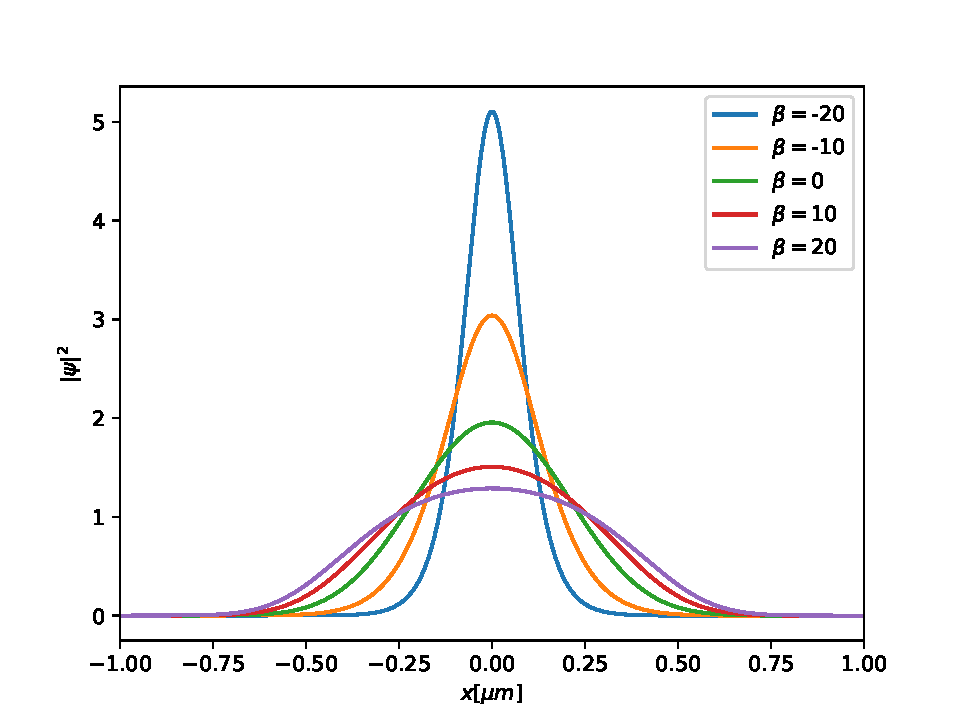
\includegraphics[width=\columnwidth]{graphics/stateAnalysis/GroundstateBeta.pdf}
	\end{subfigure}
	\begin{subfigure}{\columnwidth}
		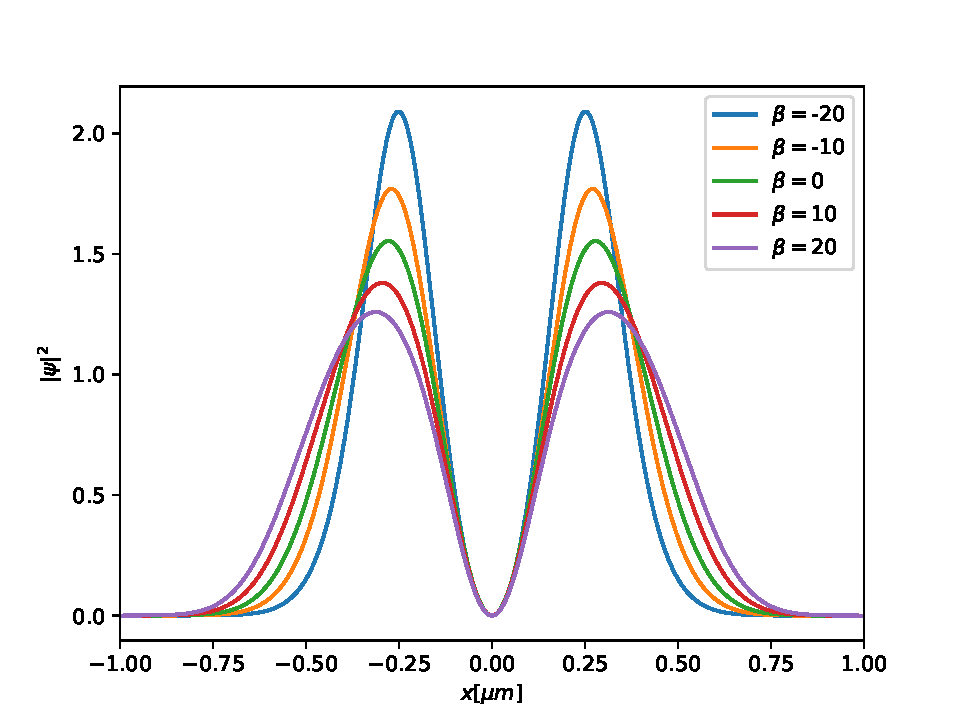
\includegraphics[width=\columnwidth]{graphics/stateAnalysis/ExcitedstateBeta.pdf}
	\end{subfigure}
	\caption{\textbf{Top:} Groundstate of a BEC in a quartic trapping potential, shown as a function of the atomic interaction parameter $\beta$ from Eq. \eqref{eq:Hbec}. \textbf{Bottom:} First excited state of the same system.}
	\label{fig:BECstates}
\end{figure}

We attempt to excite the BEC from its ground state to first excited state using a control function, usually denoted $u(t)$. The control function describes how the potential evolves in time. A simple example of this is could be that $u(t)$ could describe how a quartic potential is displaced over time:
\begin{equation}
	V(x, u(t)) = a(x-u(t))^2 + b(x-u(t))^4
\end{equation}
While it is not hard to write out \textit{some} control function, it is much more difficult to find a control that succesfully excites the initial state into the desired state. To quantify how well a given control function has performed, one can calculate the \textit{fidelity} $F = | \langle \psi_D | \psi \rangle |^2$ to calculate the overlap between the two states $\ket{\psi}$ and $\ket{\psi_D}$, where $\ket{\psi}$ is the current state and $\ket{\psi_D}$ is some desired state. Thus, the fidelity $F$ is a number between $0$ and $1$, where $0$ means that there is no overlap between the 2 states and $1$ means that the states are identical. Usually values of $0.99$ and above are set as the benchmark that a control function must satisfy. It is sometimes convenient to instead calculate the \textit{infidelity} $1-F$ to map out how well different control functions performed.\\

Since it can be very difficult to find a control function that is capable of reaching $F\approx 0.99$ and above, it is often useful to \textit{optimize} an initial control function (called a ``seed'' in this case) using different kinds of optimization algorithms. These optimization algorithms are, given enough time, usually capable of optimizing a seed into a control that can reach much higher fidelities. Regardless of which optimization algorithm is used, one must first define the optimization \textit{problem}, which is a function that the given algorithm will attempt to minimize. We define this problem as \cite{JensJacobPhDThesis} 
\begin{equation}
	\min J(u) = \frac{1}{2}(1-| \langle \psi_{t} | \psi(T) \rangle|^2) + \frac{\gamma}{2} \int_{0}^{T} \dot{u}^2 \text{d}t
\end{equation}
where $\psi_{t}$ is the target state, $\psi(T)$ is the final state evolved with the control $u(t)$ to final time $T$. The first term minimizes infidelity and the second term penalizes rapid fluctuations of the control function that can be challenging to implement experimentally. $\gamma$ is called the regularization factor and is usually on the order of $10^{-4}$ to $10^{-6}$. \\

The optimization algorithm \proc{Grape} (\textbf{Gr}adient \textbf Ascent \textbf Pulse \textbf Engineering) \cite{PhysRevA.90.033628} is available to use in both Quantum Composer and the QEngine. \proc{Grape} works by calculating the gradient of $F$ with respect to each point of a given control function on the discretized time scale 
\begin{equation}
	\vec{\nabla}_{\vec{u}}F(\vec{u})
\end{equation}
where $\vec{u} = (u(t_0), u(t_1) ... \,, u(T))$. When this calculation is done, $\proc{Grape}$ takes a step of size $\alpha_k$ such that the new discretized control function becomes
\begin{equation}
	\vec{u}_{k+1} = \vec{u}_{k} + \alpha_k \vec{\nabla}_{\vec{u}}F(\vec{u}_k)
\end{equation}
such that $F(\vec{u}_{k+1}) \geq F(\vec{u}_{k})$. This process is continued until some convergence criterium is fulfilled, e.g. a target threshold $F(\vec{u}_{k}) \geq F_{target}$, a maximum number of iterations $k \leq N$ or until the step size $\alpha_k$ becomes too small. \\

Two other optimization algorithms are available to use in the QEngine: \proc{Group} and d\proc{Group} (dressed \proc{Group}). Where \proc{Grape} is a relatively simply gradiant ascent algorithm, these two attempt to combine the local optimization that \proc{Grape} does with a global search for promising regions in the fidelity landscape \cite{GroupPaper, QEngine}. 
Note that this does not mean that an optimized seed will always be able to reach $F\approx0.99$. One particular hinderence is the \textit{Quantum Speed Limit} (QSL). This speed limit refers to the upper bound of how fast a state is able to evolve in time \cite{Deffner_2017}. This speed limit is (not surprisingly) dependent on the individual system examined and in the context of the Shake Up challenge, it refers to the minimum time required to evolve from the initial state into the target state with a fidelity of at least $F\approx 0.99$. \\

The challenge was explored in Quantum Composer by creating different systems and trying different control functions and optimization methods. The different systems had their potentials varied and the interatomic interaction parameter $\beta$ as well. The control functions themselves were varied and explored, along with the control duration $T$ and the \proc{Grape} optimization parameters $F_{target}$, $N$ and $\gamma$.


\section{Quantum Composer}\label{sec:Composer}
Quantum Composer is a tool for visualizing the behavior of a quantum mechanical system, either statically or as the system evolves in time. To do this, one combines building blocks (nodes) containing the various components (like a potential $\hat{V}(x)$) to build new nodes (like a Hamiltonian $\hat{H}$). From there, one can build a wave function from a superposition of $\hat{H}$ eigenstates using one type of node and connect it to a plotting node to have the state, its norm-square and other relevant states visualized. The system can be evolved in time using a time node. The use of Composer in this report can be grouped into three overall groups: System setup, \proc{Grape} optimization and simulation. These groups and their components have been visualized in Fig. \ref{fig:flowdiagram}. 

%TODO Redo for next report update / Thesis inclusion
\begin{figure*}
\def\svgwidth{\textwidth}
	\input{workflow.pdf_tex}
	\caption{Diagram illustrating the workflow of using Quantum Composer. Arrows indicate dependencies on other nodes. Note that nodes in the diagram do not necessarily translate directly to a node in Composer.}
	\label{fig:flowdiagram}
\end{figure*}

To simulate a quantum control problem, one first has to set up a system that describes the problem. This includes choosing boundaries of the Hilbert space and discretizing the space into a number of points. It also includes things like describing the potential of the system and the time interval $(t_0, T)$. Specifically for quantum control problems it also involves defining how the potential depends on one or multiple control functions and how these are defined. From these steps, it is then possible to build the Hamiltonian of the system and from that we can create wave functions, in particular $\psi_0$ (initial state) and $\psi_D$ (target state) that are relevant for a quantum control problem.


It is then possible to optimize the initial control function using \proc{Grape}. The optimization procedure requires a number of arguments, some optional ($\gamma$ and $\sigma$), others required ($N$ and $F_T$). The control function will then be updated until a convergence criteria is reached, after which \proc{Grape} outputs the optimized control function. In Composer it is possible to map the fidelity of the current and previous control iterations to show how fidelity improves as \proc{Grape} iterates. Likewise, it is also possible to plot the initial and current control function to see how they differ. A screenshot from Composer showing how this optimization procedure is set up can be seen in Fig. \ref{fig:composerScreens}.

\begin{figure*}
	\centering
	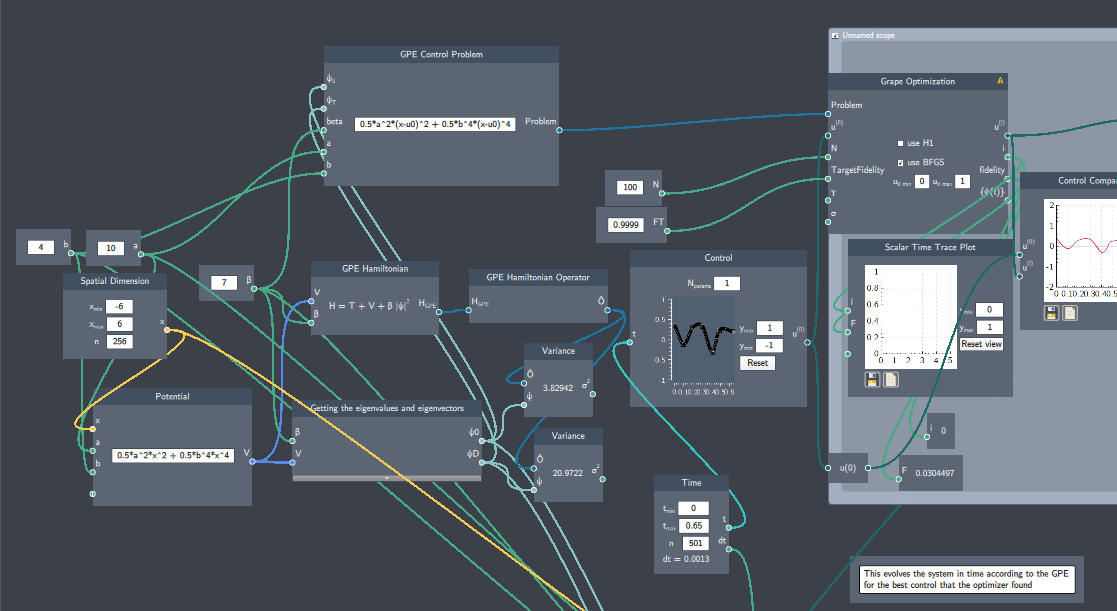
\includegraphics[width=\textwidth]{graphics/composerScreens/composerWide.png}
	\caption{Screenshot from Quantum Composer partially showing a flowfile that optimizes a control function using \proc{Grape}. The optimized solution is then simulated in a scope not shown.}
	\label{fig:composerScreens}
\end{figure*}

When the system is simulated, it is possible to analyze the wave function at the current point in time. Thus we are able to calculate and visualize different variables in our system as they are being simulated. This includes calculating the fidelity $F$ as a function of time, but we can also plot how our wave function evolves in time by mapping out $|\psi|^2(x,t)$. When the simulation is finished, the final fidelity $F(T)$ can be recorded.


The data presented in Composer, in most cases, cannot be saved directly through the program, but must instead be manually written to a separate text file. This file containing data can then be further analyzed and plotted. In this case it is done using Python and its plotting module \texttt{Matplotlib.pyplot}.


\section{Results}\label{sec:results}
\subsection{\label{subsec:numericalLimitations} Numerical limitations}
\subsubsection{Spatial resolution \& performance}
% Compare grid resolution errors
One obvious source of numerical inaccuracies is the resolution of the quantized Hilbert space one uses. Throughout the report, the spatial grid was divided into $256$ points. We can compare this resolution to other resolutions by calculating the difference between a high resolution wave function with $1024$ points and lower resolution wave functions. This difference between the different resolutions for the ground state can be seen in Fig. \ref{fig:groundstateGrid}. As can be seen in the figure we find that the lower the resolution of a wave function is, the bigger the difference between that wave function and a higher resolution one. \\
\begin{figure}
	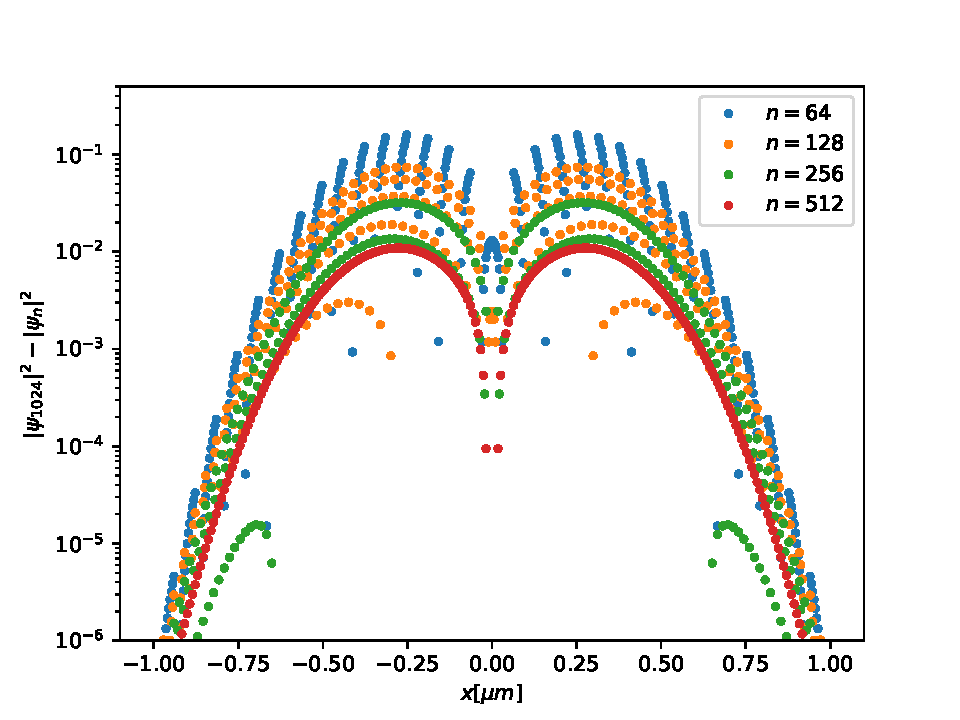
\includegraphics[width=\columnwidth]{graphics/stateAnalysis/GroundstateGrid.pdf}
	\caption{Difference between different resolutions of the initial wave function compared to a high resolution wave function.}
	\label{fig:groundstateGrid}
\end{figure}

% Relate this to time consumption to explain why we dont do use the 1024 size but instead the 256
Considering this, one would think that it would always be better to use as high spatial resolution of a given system as possible. This would of course be true if we had access to unlimited computational power. We instead have to balance the desire for a high spatial resolution and more accurate wave functions against the increased time it takes to do calculations for a higher dimension Hilbert space. As an example of this increased calculation time, a system was set up as described by System \textit{B1} seen in Appendix \ref{App:System-params}, with additional parameters: $\beta = 4$, $u(t)=0.5 \cos(2\pi t/T)$ and $T=0.8$. This system was then optimized for 100 iterations using \proc{Grape} before the system was simulated with the optimized control function. The results can be seen in Fig. \ref{fig:performanceTime}. This result confirms that choosing a grid resolution of $256$ points gives us a high accuracy compared to lower resolutions while also keeping performance time low.

\begin{figure}
	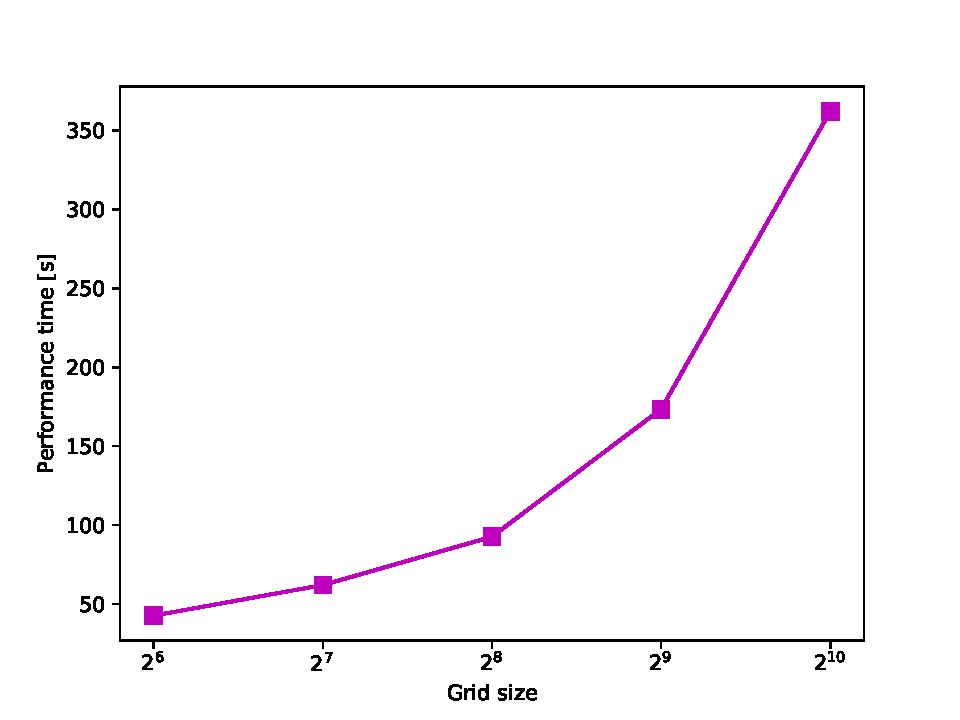
\includegraphics[width=\columnwidth]{graphics/stateAnalysis/PerformanceTime.pdf}
	\caption{The time it takes for Quantum Composer to solve the same problem as a function of the spatial grid resolution.}
	\label{fig:performanceTime}
\end{figure}

\subsubsection{Eigenvectors \& eigenvalues}

In order to obtain accurate results when making these computations, one has to ensure that the states that are analyzed are described within acceptable numerical accuracy. We can ensure that we are working with the ground state as our initial state in Composer by calculating the variance of our initial state wrt. the Hamiltonian
\begin{equation}
	\text{Var}(\psi)_H = \langle \psi \mid \hat{H}^2 \mid \psi \rangle - \left(\langle \psi \mid \hat{H} \mid \psi \rangle\right)^2
\end{equation}

This gives us a numerical estimate of how ``close'' our initial state is to the actual ground state of $\hat{H}_{GPE}$ since
\begin{equation}
	\psi \text{ is an eigenstate of } \hat{H}_{GPE} \iff \textsc{Var}(\psi)_H = 0
\end{equation}

The way the energy spectrum of $\hat{H}_{GPE}$ is calculated is not trivial \cite{QEngine}, but the variance can generally be reduced by adjusting different parameters of the system or Composer file, e.g. spatial dimension $x$ or initial conditions for the $H_{GPE}$ spectrum node. Despite these possible fixes, the numerical limitations of Quantum Composer become apparent as the ``Shake Up'' problem is explored in increasingly greater details and limits and accuracy are pushed further and further. The following paragraphs describe areas where the numerical limitations are significantly limiting the exploration of certain aspects of this problem.\\

As the work with the QSL shown in Fig. \ref{fig:QSL} was explored, it was desirable to examine how the energy levels of the state changed as a function of $\beta$. The idea was that $\beta$ could change the spacing between the different levels of the potential well and perhaps further increase the energy separation for some high or low values of $\beta$. As was shown in Fig. \ref{fig:HO}, the even spacing of a quadratic potential makes it difficult to reach the high fidelities desired. To investigate this, the energy difference between the first excited state and the ground state as well as the difference between the second and first excited state was calculated in Composer. %TODO Carrie says its even impossible, read feedback 3 and rewrite 
Even though Composer is unable calculate the second excited state of a BEC, it was also desired to explore how the ground and first excited state energies changed as a function of $\beta$. These energies are plotted in Fig. \ref{fig:energyLevels} and as can be seen, the uncertainty in the excited states increase for values of $\beta$ below $-10$. As mentioned when estimating the optimizable limit of negative $\beta$'s, this could explain why $\beta=-10$ is the optimizable limit found.\\

\begin{figure}
	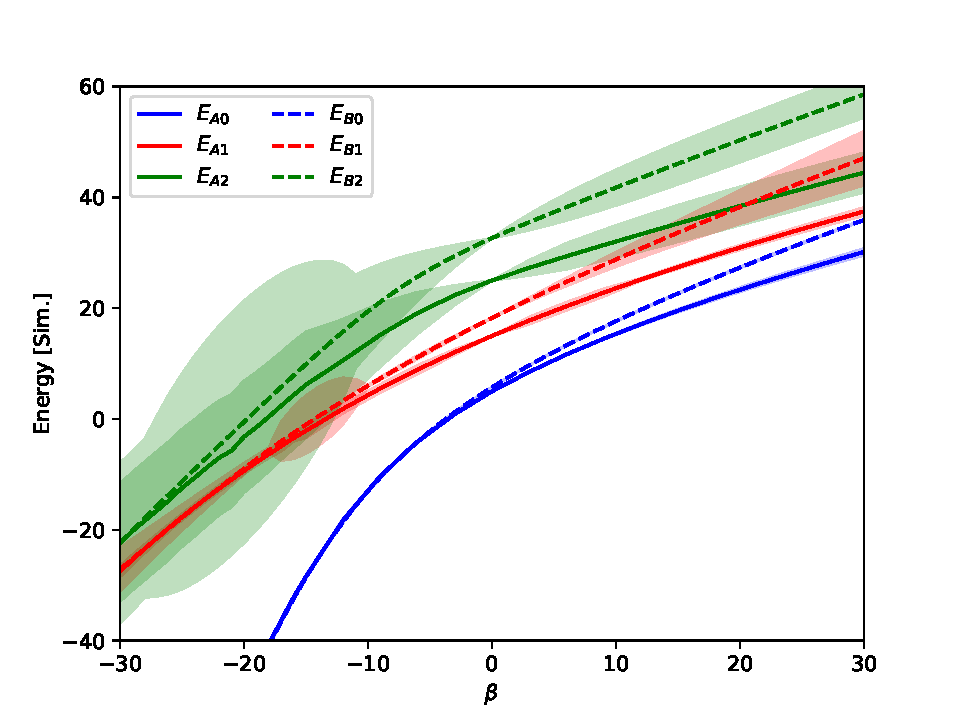
\includegraphics[width=\columnwidth]{graphics/stateAnalysis/Energylevels.pdf}
	\caption{Calculated energies of the first 3 energy eigenstates of a BEC in a quatic potential as a function of $\beta$.}
	\label{fig:energyLevels}
\end{figure}

Even when working within the low-variance range of this problem, one still has to be careful of numerical errors caused by the control function used. These problems with the control function seem to be caused by a combination of different factors:
%TODO: How high is high and why does large durations mess up? Is is bc of build up of numerical error (most likely, but pls verify) or something else?
1. Using ``high'' frequency control functions. 2. Initial control functions having large displacements. 3. Larger control durations. As an example, one can see how the $k=4$ seed from Fig. \ref{fig:Clustering} performed for a duration of $T\approx 0.85$ms compared to a $k=5$ with longer duration  $T\approx 1.0$ms with a smaller amplitude. The comparison can be seen in Fig. \ref{fig:statePlots} where the resulting state evolution of each of these optimized seeds are shown. The consequence of this error is that the control space that is possible to explore in Composer is limited to what can be handled without breaking the state due to inaccuracy. Thus, high frequency controls can be explored, but if sufficiently large durations are desired, then the amplitude of this oscillation must be scaled to accommodate this.
%TODO Re-read page 5 of Carries feedback for report 3 to check this is solved for next handin

\begin{figure}
	\begin{subfigure}{0.45\columnwidth}
		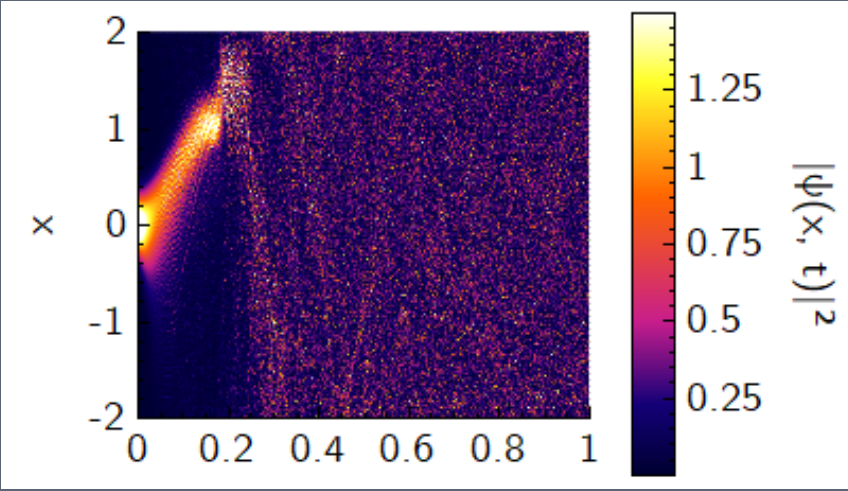
\includegraphics[width=\columnwidth]{graphics/clustering/QM2Clusteringk4A04T06178-2.PNG}
	\end{subfigure}
	\begin{subfigure}{0.45\columnwidth}
		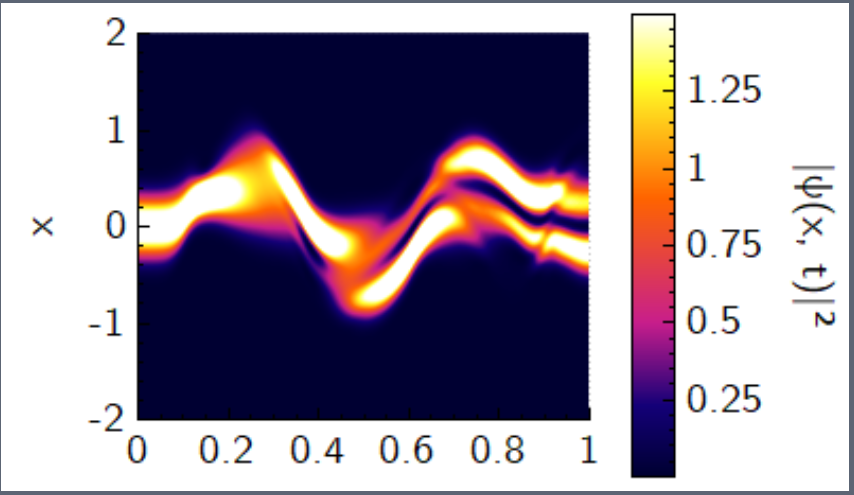
\includegraphics[width=\columnwidth]{graphics/clustering/QM2Clusteringk5A015T07475-2.PNG}
	\end{subfigure}
	\caption{Comparison of the state evolution for a numerically broken state (left) and a numerically working state (right). On the first axis is normalized control time and on the second axis position in $\mu$m.}
	\label{fig:statePlots}
\end{figure}

% BEC in harmonic
\subsection{Harmonic potential optimization}
%TODO Reproduce energy spec. for quadratic potential to show that non-lin contribution to H makes shaking better
%TODO Mention that this is system A1
Due to the equally spaced energy levels of a quadratic potential, it is difficult to excite the state exclusively to the first excited state. It is likely that some part of the state is driven into higher excited states and so it is challenging to reach high fidelities with this kind of potential. Nonetheless, the nonlinear contribution to the GPE Hamiltonian seems to make it possible to improve the fidelity of control functions compared to the levels reachable for a single particle. In a quadratic potential different controls were optimized to estimate the highest reachable fidelity for this kind of potential as a function of the nonlinear interaction strength $\beta$. These controls were optimized with \proc{Grape} for $100$ iterations and the highest reachable fidelity was then noted. The results can be seen in Fig. \ref{fig:HO}. As can be seen on the figure, it is actually possible to reach higher levels of fidelity for all measured values of $\beta \neq 0$ with control duration $T = 1$. The highest result shows that it is possible to improve the fidelity score with about $50\%$ compared to the reachable score of a single particle. One should also note that controls with duration $T=7.5$ do not perform as well as the other 2 shown durations. This is suspected to be caused by the long control duration allowing for states to be excited beyond the targeted first excited state, which the smaller control durations are not as susceptible to. Another explanation could be that the increased control duration makes the optimization landscape more complex and so more sensitive to the inital control that is being optimized on.

\begin{figure}[h]
	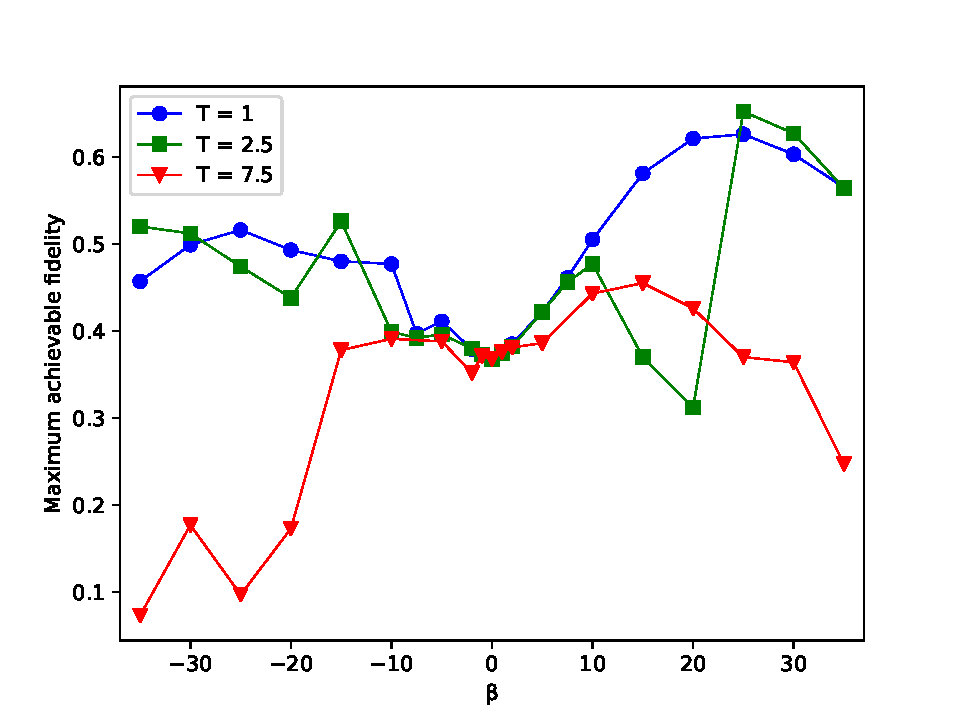
\includegraphics[width=\columnwidth]{graphics/exploration/betaTHO.pdf}
	\caption{The result of varying $\beta$ and $T$ for a BEC in the harmonic potential. There exists combinations where it is possible to achieve above $50\%$ higher fidelity compared to a single particle (at $\beta=0$), but many also combinations also perform worse than for a single particle.}
	\label{fig:HO}
\end{figure}

\subsection{Unoptimized BEC control in a quartic potential}

% BEC in anharmonic
%TODO Mention that this is B1
Through simulations it seems that BECs have very different dynamics compared to single particles. Without using $\proc{Grape}$, one can study how the similarity between single particles and BECs changes depending on the value of $\beta$. Keeping the control function and control duration the same, we find that what was a good solution for a single particle reaches a lower and lower fidelity as we change $\beta$ away from 0, but that it also reaches revivals with a higher fidelity compared to neighboring values. This behavior is shown in Fig. \ref{fig:beta} where the non-optimized control
\begin{equation}
	u_{\mathrm{non-opt}}(t)=0.12\cdot\sin(0.86\cdot \omega_{01} t)
	\label{eq:nonopt-control}
\end{equation} with final time $T=3.49$ was simulated for different values of $\beta$. We define $\omega_{01}$ to be the energy frequency between the ground and first excited state. This varying should not come as a surprise. The function in Eq. \eqref{eq:nonopt-control} was chosen because of its high fidelity score around $\beta=1$, but expecting this control function to perform well for the wide range of other systems (i.e. values of $\beta$) it is tested on would not be expected. While the behavior of similar systems is not vastly different, this small change to the system dynamics does mean that some systems will not reach a high fidelity at the final time, while others will. This can also be seen in Fig. \ref{fig:fidelityplot}, where the fidelity as a function of time has been plotted for 2 different interaction strengths. 
In conclusion, using a single, non-optimized control for a broad range of systems is not viable, as success boils down to timing whether or not the control terminates at a high fidelity.

\begin{figure}[h]
	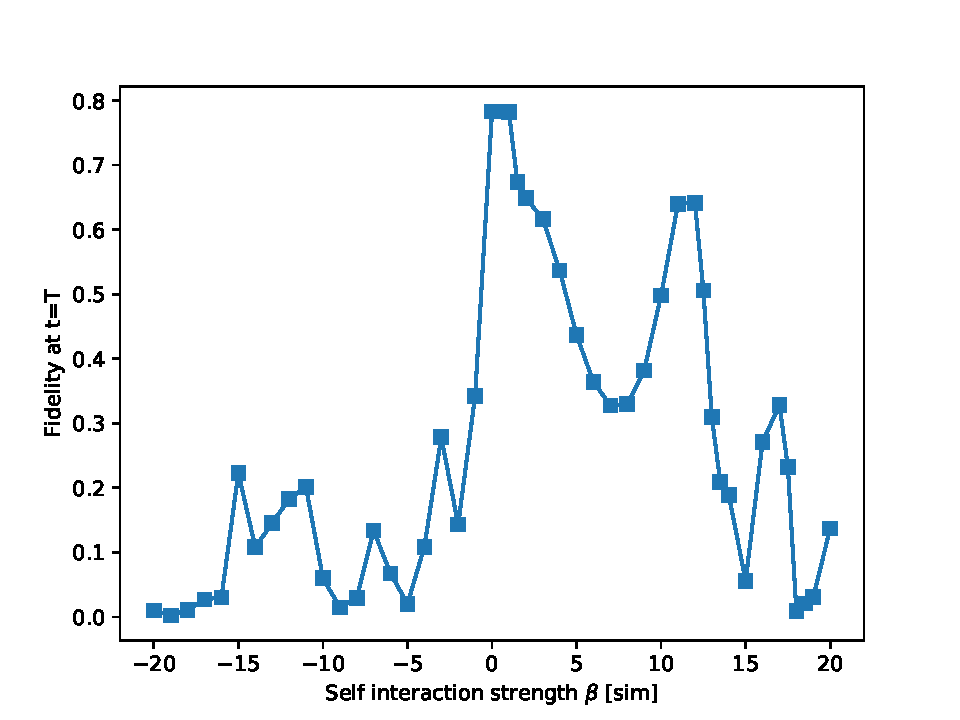
\includegraphics[width=\columnwidth]{graphics/exploration/nonOptBeta.pdf}
	\caption{Fidelity of a non-optimized solution for different values of $\beta$ in a quartic potential.}
	\label{fig:beta}
\end{figure}

\begin{figure}
	\begin{subfigure}{0.45\columnwidth}
		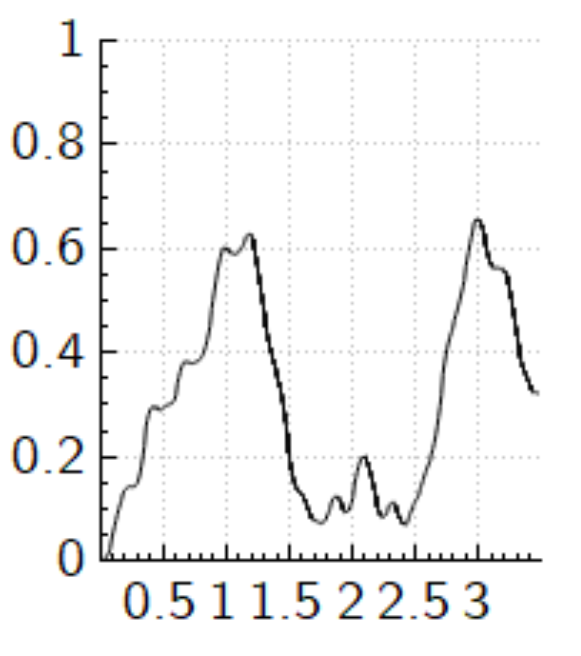
\includegraphics[width=\columnwidth]{graphics/exploration/betaNonOptFidelityBeta7.PNG}
	\end{subfigure}
	\begin{subfigure}{0.45\columnwidth}
		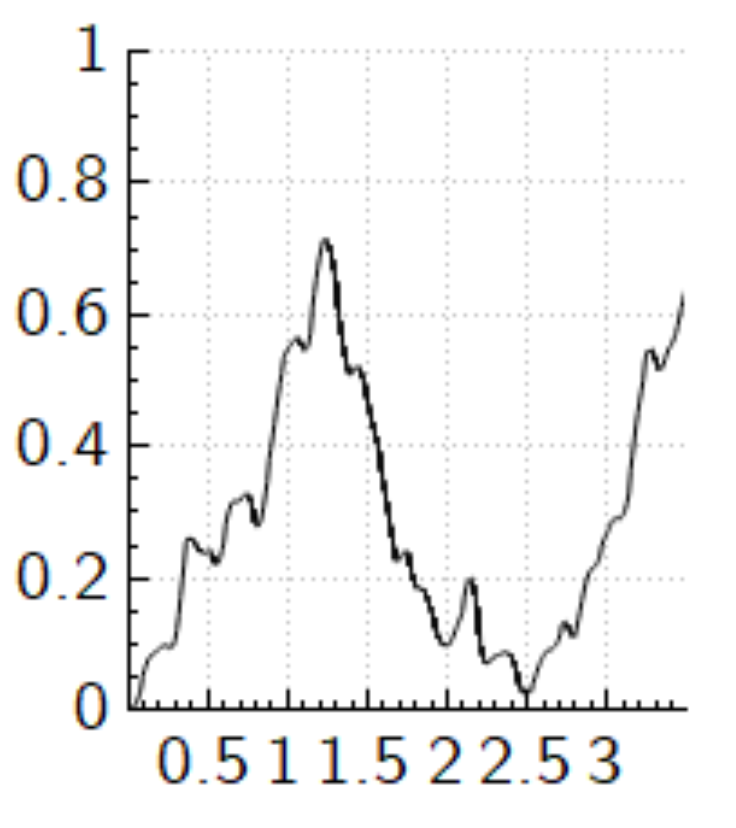
\includegraphics[width=\columnwidth]{graphics/exploration/betaNonOptFidelityBeta12.PNG}
	\end{subfigure}
	\caption{Fidelity as a function of time for the control function in Eq. \eqref{eq:nonopt-control} for two different values of $\beta$. Left is $\beta=7$, right is $\beta=12$. As can be seen, the overall trend is the same for the 2 systems and so it becomes a matter of 'timing' the final time to reach a higher fidelity if one refrains from using \proc{Grape} to optimize controls.}
	\label{fig:fidelityplot}
\end{figure}

\subsection{Quantum speed limit}
%QSL
%TODO This is also system B1
It was attempted to estimate the Quantum Speed Limit for this control problem and its dependence on the interaction strength of the BEC, $\beta$. The system parameters used are described under \textit{System B1} in Appendix \ref{App:System-params}. The methods for determining seeds are discussed in section \ref{sec:strats}. The seeds chosen were then optimized for 100 iterations in order to estimate the duration above which optimized controls reach a fidelity of $0.99$. The resulting estimates of the QSL for different values of $\beta$ can are shown in Fig. \ref{fig:QSL}. Notice how it seems that the speed limit is lower for attractive BECs and increasingly higher for increasingly more repulsive BECs. It was not possible to estimate the QSL for values of $\beta$ below $-10$ or above $25$, since no control function could be optimized to $0.99$ within 100 iterations. \\

\begin{figure}[h]
	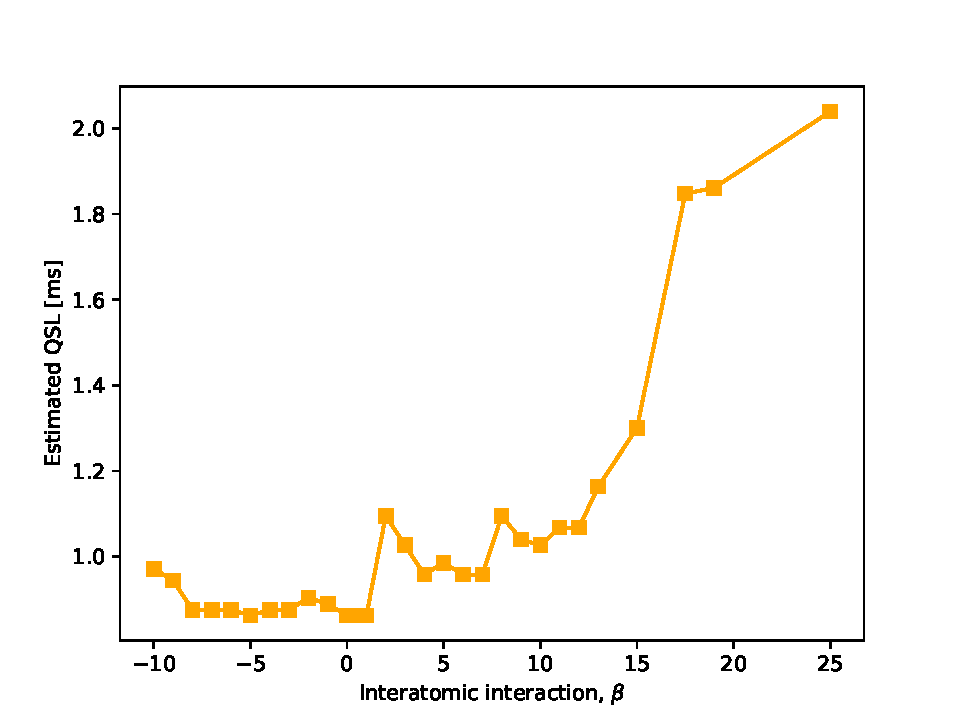
\includegraphics[width=\columnwidth]{graphics/exploration/QSL.pdf}
	\caption{The estimated Quantum Speed Limit for a BEC in a quartic potential as a function of $\beta$.}
	\label{fig:QSL}
\end{figure}

\subsection{Optimizable lower bound of $\beta$}

It is clear after having explored the behavior of BECs in different numerical setups that the behavior the BECs are not symmetric with respect to $\beta$. This is not unexpected, since the sign of $\beta$ constitutes whether the atom-atom interaction happening inside the BEC is repulsive($\beta>0$) or attractive ($\beta<0$) and so it would not be unjustified to say that the sign of $\beta$ describe entirely different species of bosons. Since attractive BECs have proven difficult to optimize on for $\beta<-5$, it was explored what the lower limit of $\beta$ would be with respect to reaching an optimizable fidelity of at least $0.99$. The results of this exploration is seen in Fig. \ref{fig:reachable_neg_betas}, where it can be seen that for values of $\beta<-10$ it is no longer possible to reach $F\geq0.99$. While this lower bound could be seen as a numerical limitation of Composer as discussed in Sec. \ref{subsec:numericalLimitations}, it is also relevant to consider that there exists a lower bound for how attractive a BEC can be before the atoms collapse in on themselves in a process known as a Bose-Nova \cite{Donley2001}.


\begin{figure}
	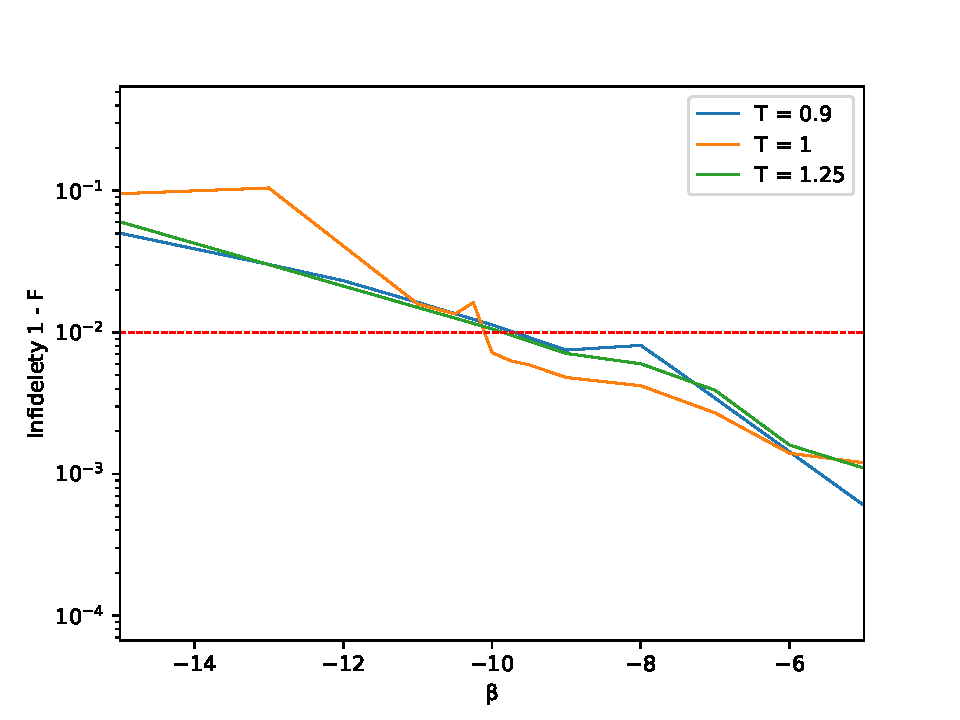
\includegraphics[width=\columnwidth]{graphics/exploration/reachable_neg_beta.pdf}
	\caption{Lowest reachable infidelities as a function of interatomic attraction $\beta$, shown for different timescales. It seems that $\beta=-10$ is the lower limit for reaching optimizable solutions $F\geq0.99$. This lower limit is, however, suspected to be caused by numerical inaccuracies. The dashed red line marks where the fidelity of a control is $0.99$.}
	\label{fig:reachable_neg_betas}
\end{figure}

%clustering of solutions
\subsection{\label{subsec:clustering}Clustering of solutions}

In a recent article \cite{QM2Paper} where this problem has also been studied, it was found that optimal solutions for increasing final times were dominated by cosine functions of increasing frequencies $k\pi t/T$. The figure from Ref.  \cite{QM2Paper} showing this is shown in Fig. \ref{fig:Clustering}

To replicate this result using Quantum Composer, the system conditions had to be rescaled to Composer, where the kinetic factor $\kappa$ is locked at $0.5$, while in the original system it was instead $0.36537$. Thus, the different quantities of the system had to be reworked. This recalculation can be seen in Appendix \ref{App:System-params}. \\

It was attempted to replicate this result by letting \proc{Grape} optimize seeds of the form $u(t) = A\cos(k\pi t/T)$ for 750 iterations each. By varying $k$ and $A$, the frequency and amplitude of the seeds were varied and their optimized solutions and reached fidelity noted. The results can be seen in Fig. \ref{fig:Clustering}. As can be seen on the figure, the results do not replicate those found in Ref. \cite{QM2Paper} where solutions dominated by different values of $k$ outperform other $k$'s for some interval. Note in particular that the overall highest fidelity was reached for a seed with frequency $k=2$ at $ T\approx 0.93 \text{ms} $, where $ k=5 $ was expected to be the best performing frequency. However, note that both $k=4$ and $k=5$ reach solutions that outperform the other seeds for that particular timescale and that they do so in the expected order (4 before 5). 

%TODO Update this paragraph once it is known in more detail what causes state breakings
As is also shown on the figure, seeds with different frequencies do not have the same amplitude. The reason for this is that as the frequency of the seeds increased, it was found that having a too high amplitude caused the state to become numerically unstable and the simulation to not function correctly. This is also the reason that the $k=4$ data spans a smaller time interval due to numerical errors in their solutions for $T>0.8 ms$. \\

\begin{figure}
	\begin{subfigure}{0.9\columnwidth}
		\centering
		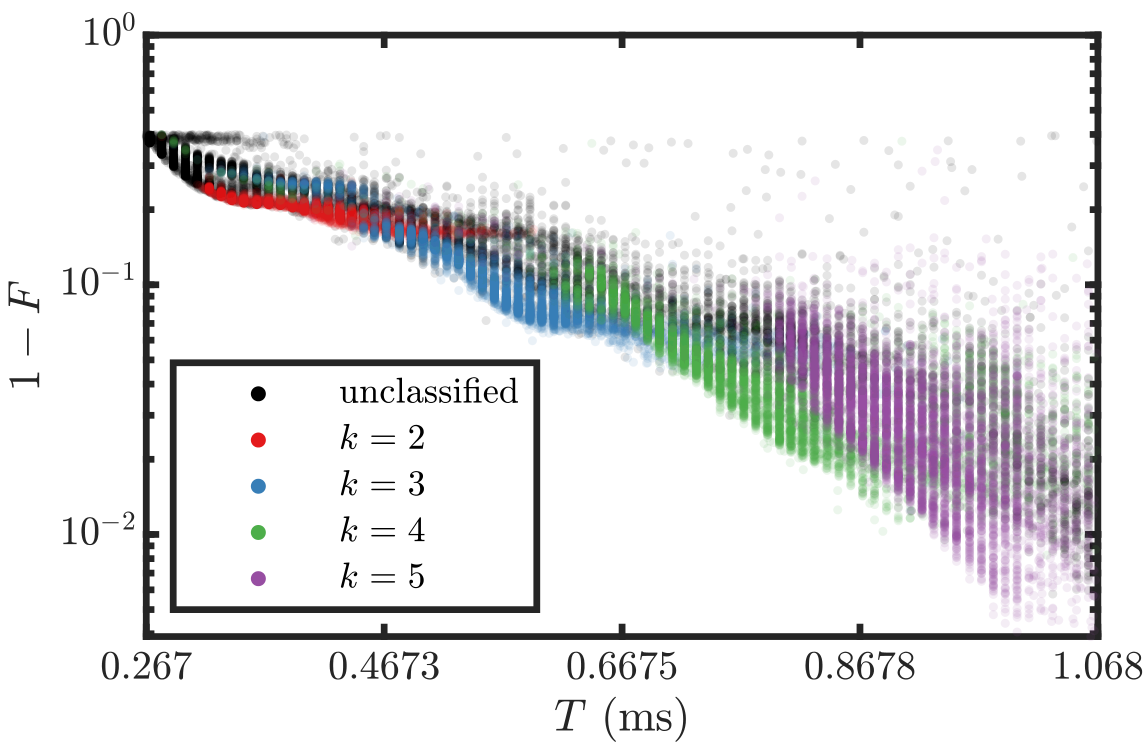
\includegraphics[width=\columnwidth]{graphics/clustering/QM2Screenshot.png}
	\end{subfigure}
	\begin{subfigure}{\columnwidth}
		\centering
		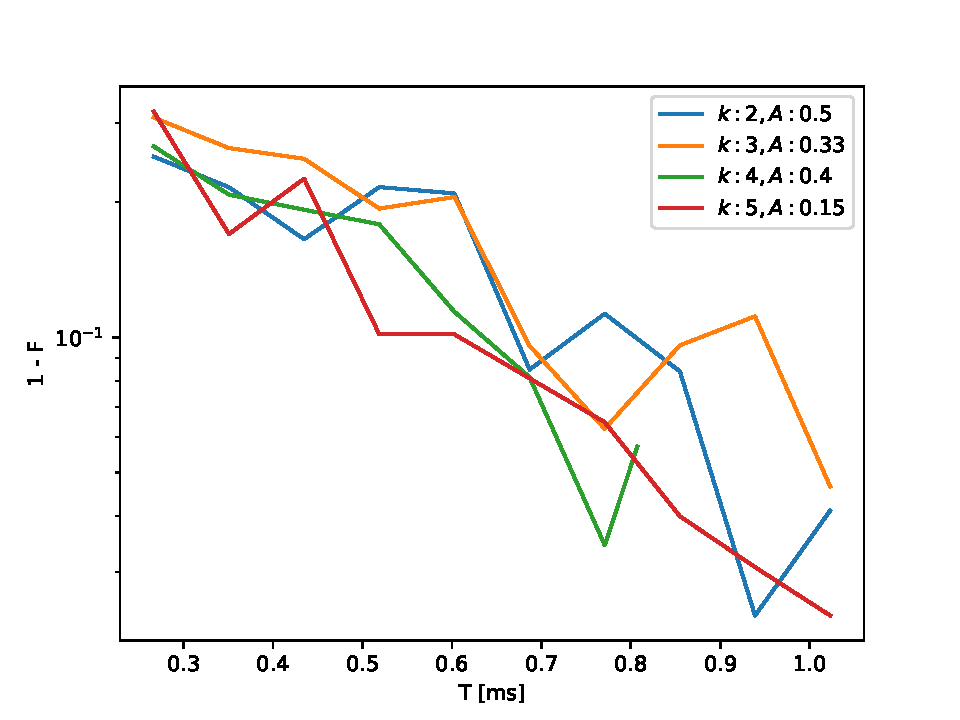
\includegraphics[width=\columnwidth]{graphics/clustering/QM2Clustering.pdf}
	\end{subfigure}
	\caption{
		\textbf{Upper}: This figure is taken from \cite{QM2Paper} and shows how optimized controls can be clustered by their projection onto $\cos(k\pi t/T)$. \textbf{Lower}: Infidelity of \proc{Grape} optimized solutions with initial control $u(t)=A\cos(k\pi t/T)$. The first axis shows the control duration $T$.}
	\label{fig:Clustering}
\end{figure}


As can be seen in Fig. \ref{fig:Clustering}, there are durations where the different control seeds reach similar levels of fidelity. This could indicate that they find the same or a similar optimized solution. The optimized solutions from Fig. \ref{fig:Clustering} with control duration $T\approx 0.685$ms are shown in Fig. \ref{fig:similarSolutions}. As can be seen on this figure, these optimized controls do not look alike despite reaching similar fidelities. It is most likely due to how different their initial control seeds are and so, one could argue that these seeds are located away from each other in the fidelity landscape. %TODO Note here that QM2 paper found Shake up to be the most complex landscape

%TODO Rewrite once the definition of a shake is more clear
What should be noted though is the connection between seed frequency in $k\pi$ and the number of 'shakes' on the corresponding optimized control function. We see that for $k=2,3,4$ the number of shakes matches this frequency, which also strengthens the hypothesis for why these seeds don't converge to the same control. \\

\begin{figure}
	\begin{subfigure}{0.4\columnwidth}
		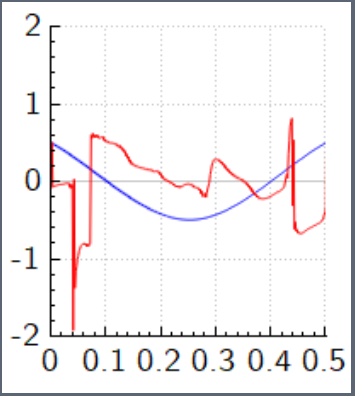
\includegraphics[width=\columnwidth]{graphics/similar_solutions/k2.PNG}
		\caption{$k=2$}
	\end{subfigure}
	\begin{subfigure}{0.4\columnwidth}
		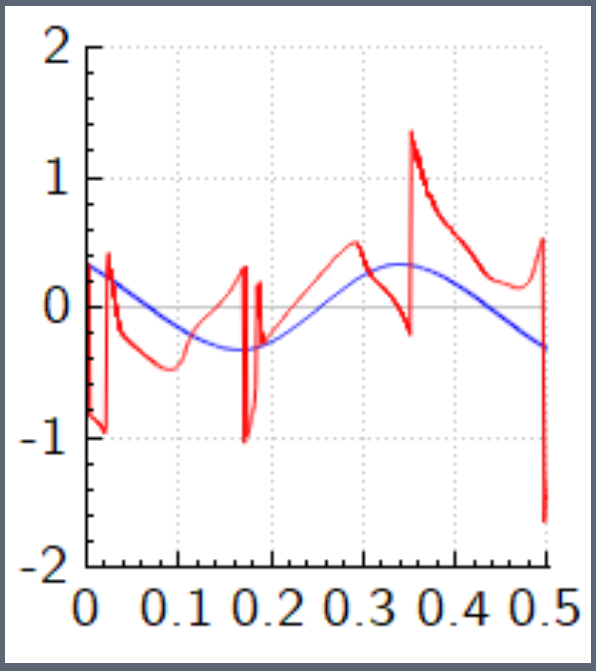
\includegraphics[width=\columnwidth]{graphics/similar_solutions/k3.PNG}
		\caption{$k=3$}
	\end{subfigure}
	\begin{subfigure}{0.4\columnwidth}
		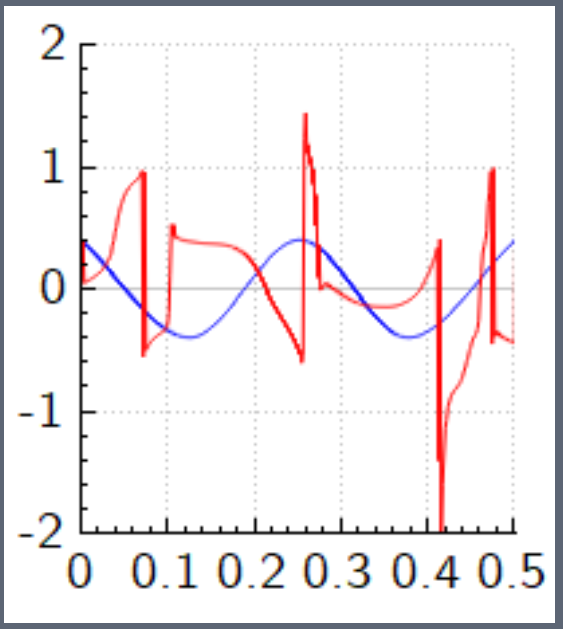
\includegraphics[width=\columnwidth]{graphics/similar_solutions/k4.PNG}
		\caption{$k=4$}
	\end{subfigure}
	\begin{subfigure}{0.4\columnwidth}
		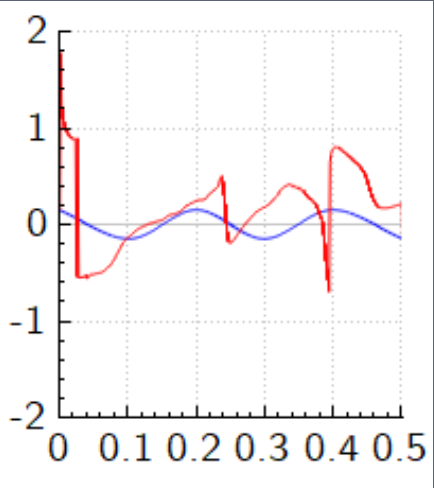
\includegraphics[width=\columnwidth]{graphics/similar_solutions/k5.PNG}
		\caption{$k=5$}
	\end{subfigure}
	\caption{Screenshots from Quantum Composer showing \proc{Grape} optimized controls for the same seeds as in Fig. \ref{fig:Clustering}. First axis is time in scaling units, second axis is potential displacement from $x=0$ in scaling units. Each figure shows the control seed (blue) and \proc{Grape} optimized control (red) for that seed.}
	\label{fig:similarSolutions}
\end{figure}

%TODO Rewrite this once shake def is in order
While examining the optimized solutions it was found that seeds with the same frequency in $k\pi$ would sometimes converge to similar optimized controls. An example of this is shown in Fig. \ref{fig:SimilarTimescales}, where the seed $A\cos(3\pi t/T)$ was optimized for different amplitudes $A$ and different durations $T$, yet still reached a very similar optimized solution. Notice also that both of these solutions have 2  shakes in the regime where it was found that optimal solutions were dominated by $\cos(2\pi t/T)$ frequencies \cite{QM2Paper}.

\begin{figure}
	\begin{subfigure}{0.4\columnwidth}
		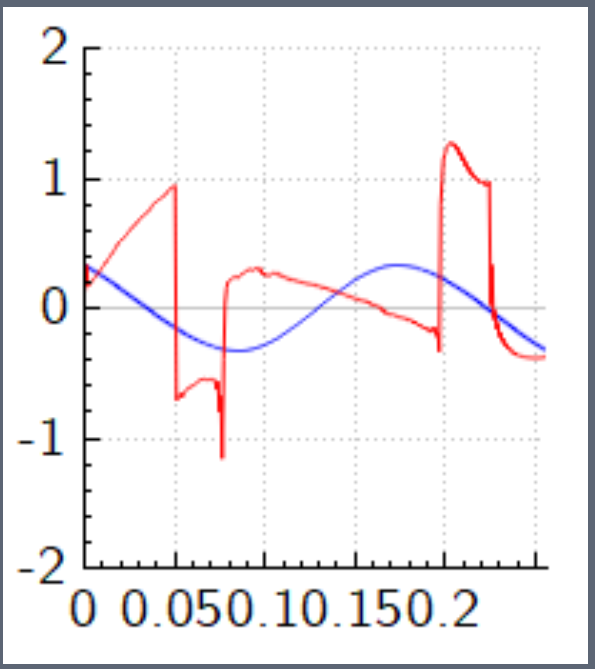
\includegraphics[width=\columnwidth]{graphics/similar_solutions/T02563k3A033.PNG}
	\end{subfigure}
	\begin{subfigure}{0.4\columnwidth}
		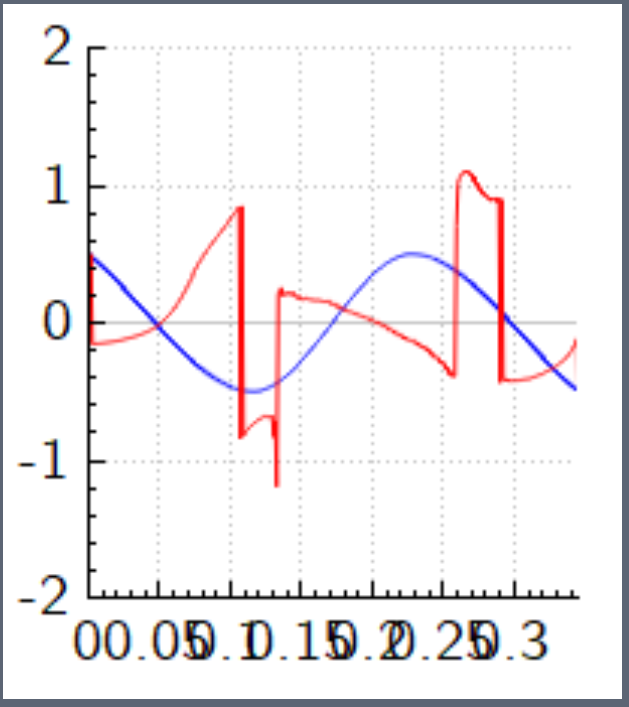
\includegraphics[width=\columnwidth]{graphics/similar_solutions/T03450k3A050.PNG}
	\end{subfigure}
	\caption{Screenshots of optimized controls of a similar seed for 2 different durations. The axis are read in the same way as in Fig. \ref{fig:similarSolutions}. Left: $T\approx 0.35$ms, $A=0.33$. Right: $T\approx 0.47$ms, $A=0.50$.}
	\label{fig:SimilarTimescales}
\end{figure}

\subsection{\label{subsec:robustness} Robustness of solutions}
The robustness of optimized solutions wrt. interaction strength or potential scaling was studied in \cite{GroupPaper}. This is interesting since real experiments are often subject to the inherent uncertainties of their equipment e.g. the frequency width of a laser. Since the interatomic interaction in a BEC is dependent on the number of atoms it consists of, it is not surprising that a specific factor $\beta$ is difficult to replicate exactly in the lab. Likewise the trapping potential is created by standing waves of laser light and so it is also subject to some uncertainty in intensity and frequency.  \\
%TODO Mention explicitly that what I mean by sensitivity is fractional change and not the point at which fidelity crosses some threshold
The robustness of optimized solutions was explored using the Composer implementation of Quantum Moves 2 (see Appendix \ref{App:System-params} for details). This replication was done by letting \proc{Grape} optimize the same control seed, $u(t)=0.15\cos(5\pi t/T)$, for $300$ iterations and for different durations $T=0.5$, $T=0.875$ or $T=1.3$, noting that these durations are respectively below, near and above the QSL of this system. These optimized solutions were then replayed in a system with a modified interaction strength $\tilde{\beta} = a_I \beta$ or in a system with a modified potential $\tilde{V}(x,u(t)) = a_V V(x,u(t))$. The results can be seen in Fig. \ref{fig:robustness}. As can be seen on the figure, there seems to be an overall trend where the more optimized a solution is for the system, the more sensitive it is to small changes in either the potential or the interaction. Keeping in mind that better solutions are reached for longer durations, this could also be intepreted as how the 'fidelity landscape' becomes increasingly more complex the longer the control duration is. This could make sense since for small durations below the QSL, there could be many 'plateaus' near optimal fidelity. Small changes to the system would change the shape/height of the plateau, but if the changes are small then the optimized solution should still be somewhere on this plateau. On the contrary, for long durations above the QSL, the landscape is more ``spiked'' due to some specific solutions being able to reach very high fidelities and this spiked landscape would of course be more affected of changing parameters. \\
%TODO Also include POV of how landscape changes from Mogens / Jesper Mohr talk


\begin{figure}
	\begin{subfigure}{\columnwidth}
		\centering
		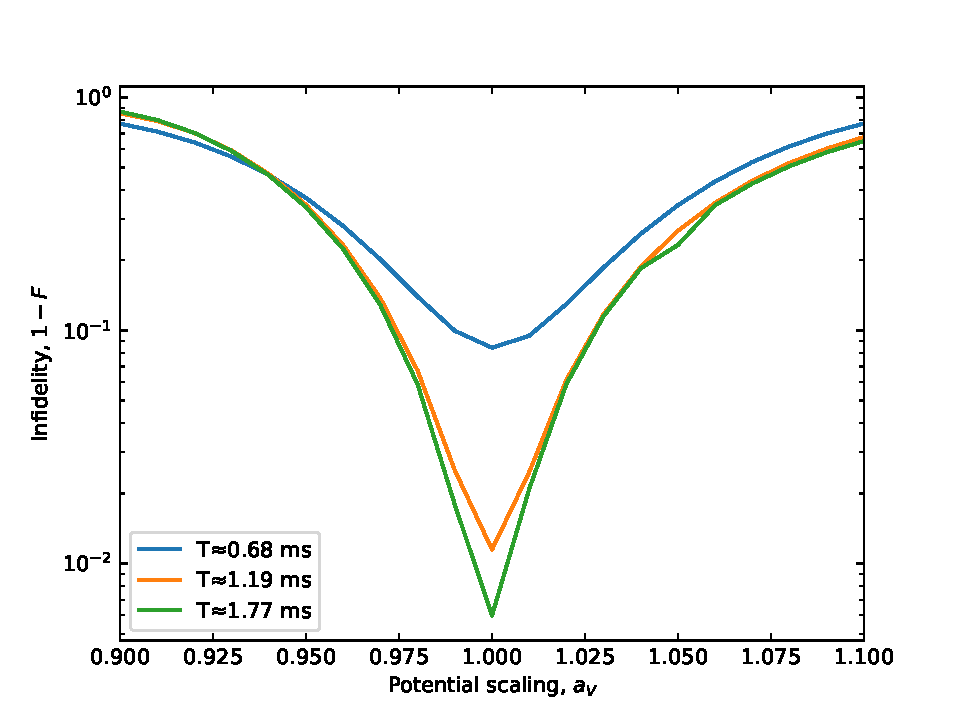
\includegraphics[width=\columnwidth]{graphics/robustness/robustness.pdf}
	\end{subfigure}
	\begin{subfigure}{\columnwidth}
		\centering
		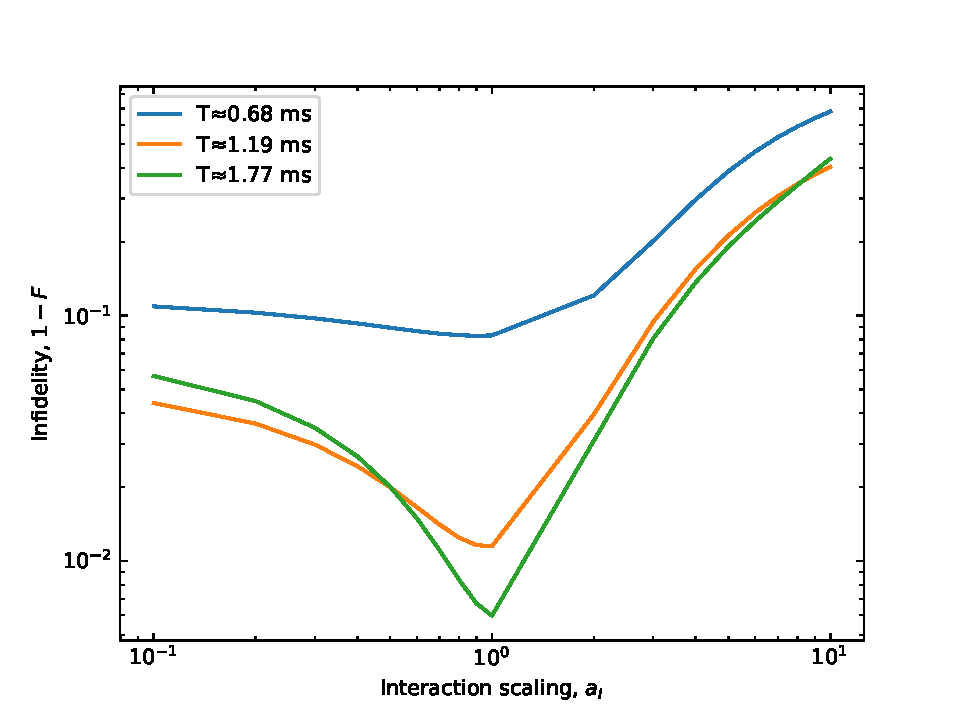
\includegraphics[width=\columnwidth]{graphics/robustness/interactionRobustness.pdf}
	\end{subfigure}
	\caption{Examining the robustness of an optimized solution wrt. scaling either the potential (top) or the atomic interaction (bottom).}
	\label{fig:robustness}
\end{figure}


\section{Strategies}\label{sec:strats}
% Function vs graph approach
Throughout working with this project, there has been two ways to determine the control function $u(t)$ in Composer: The control function is determined either by an analytical expression (using the Scalar expression node) or it is made by dragging the desired ``path'' of displacement on a graph (using the Control node). These different nodes are shown in Fig. \ref{fig:Controls}. One can use both of these approaches when working with quantum control and they both have their advantages and disadvantages. \\

\begin{figure}[h]
	\begin{subfigure}[b]{0.4\columnwidth}
		\centering
		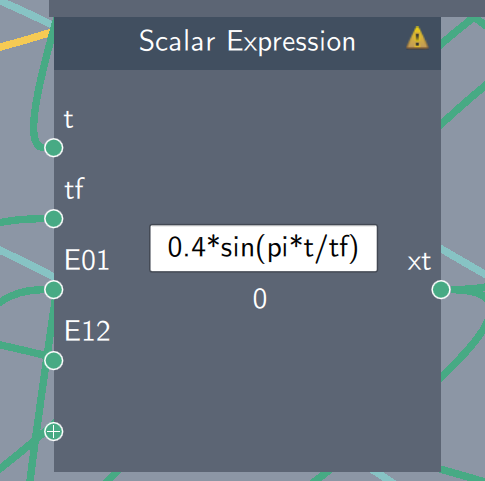
\includegraphics[width=\columnwidth]{graphics/composerScreens/ScalarExpressionNode.png}
		\caption{Scalar expression node}
	\end{subfigure}
	\hfill
	\begin{subfigure}[b]{0.45\columnwidth}
		\centering
		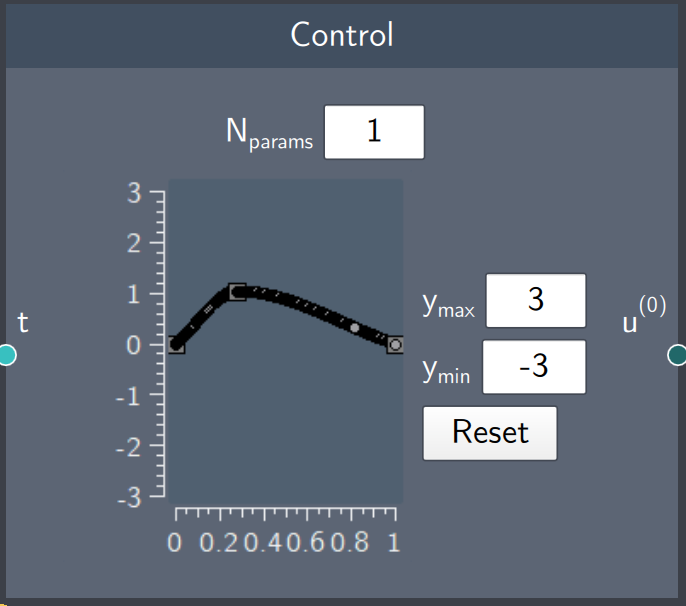
\includegraphics[width=\columnwidth]{graphics/composerScreens/ControlNode.png}
		\caption{Control graph node}
	\end{subfigure}
	\caption{Both nodes used for making a control function in Quantum Composer. The analytical function method (a) can take a number of input constants like final time $tf = T$, energy spacing between different states $(E01 = E_1 - E_0)$ and variables such as time $t$. The graph method (b) always scales the first axis such that the first point on the graph is at $t=t_0$ and the final point is at $t=T$.}
	\label{fig:Controls}
\end{figure}

% About function approach
Using an analytical expression as a control function, one gets the possibility of tweaking initial parameters to great accuracy such that the seed $\proc{Grape}$ gets already has a high fidelity. It is preferable to the graph approach in cases where a desired oscillation frequency is wanted e.g. the function $A\sin(E_{01}t)$. These kind of functions are difficult to mimic in the graph approach. When working with expressions independent of the final time $T$, adjusting this parameter translates into cutting the graph at different times. This is useful when exploring different functions and one finds that higher fidelity occurs at a different time than one currently works with. This method is shown in Fig. \ref{fig:funcAppr}. \\
\begin{figure}
	\def\svgwidth{\columnwidth}
	\input{graphics/strategies/functionAppr.pdf_tex}
	\caption{This figure shows how using an analytical control function can be used to reach a higher fidelity seed by altering the final time $T$. In this example we use the control function shown in red and the final time $T_1$. Evolving the system for a shorter(longer) time yields a higher fidelity though, and we can reach these fidelities by replacing the final time with $T_2$ ($T_3$). This method only works if the control function is independent of the final time.}
	\label{fig:funcAppr}
\end{figure}

% About graph approach
The Control graph node makes it possible to build up the control function as a series of steps. Here one can move one point on the graph and watch how the state evolves until that point, making it possible to optimize each step before going further. Since the graph node always spans the entire time interval $\{t_0,T\}$, this makes using the node useful when wanting to stretch or contract the entire function as shown in Fig. \ref{fig:graphAppr}. As demonstrated with the BEC in a harmonic potential in Fig. \ref{fig:HO}, there exists a complex relationship between $\beta$ and $T$ and so being able to keep the shape of the control function the same while altering the total time makes the node a beneficial tool to use.\\

\begin{figure}
	\def\svgwidth{\columnwidth}
	\input{graphics/strategies/graphAppr.pdf_tex}
	\caption{A visualization of one method that can be used to optimize fidelity when working with the graph node. If one tries to change the final time $T$ the resulting control function will be squeezed or stretched as a result. Altering the final time can be beneficial given the complex relationship between $\beta$ and $T$, but also as a tool to regulate the speed at which the potential moves. Using this approach also has the practical advantage that we can draw the graph such that $u(T)=0$ and so no matter the final time, the potential will always end up where it started. This is to be compared to the approach shown in Fig. \ref{fig:funcAppr} where this is not always the case and the state would possibly need to be transported back to its initial position.}
	\label{fig:graphAppr}
\end{figure}

When calculating the maximum reachable fidelity for some combination of $\beta$ and $T$ in the harmonic potential, the graph control node was used to seed the $\proc{Grape}$ algorithm. The overall strategy using this tool involved moving points on the graph into certain shapes and looking at how the initial (i.e. no $\proc{Grape}$) fidelity looked. I particularly liked the semi-circle shape of a $\sin(\pi t/T)$ function where the amplitude was varied. Another particular shape used in this work was generated by moving a single point around $0.1T$ or $0.9T$ to create a function which had a fast(slow) buildup to a maximum and then a slow(fast) return to the initial position. This wedge-like shape is shown in Fig. \ref{fig:Controls} (b).

Both of these strategies worked well and provided nice seeds for $\proc{Grape}$ to optimize on. Despite some cases where the fidelity changes significantly from small variations of $\beta$, the overall rule seems to be that something that works well for one value of $\beta$ will have a similar fidelity for nearby values of $\beta$, and so this was also used to find a good seed when $\beta$ was larger than $10$, since above this limit the system seemed a lot more sensitive to the initial control function with respect to reaching the highest possible fidelity for that particular combination of $\beta$ and $T$. \\

Measuring the Quantum Speed Limit for the quartic system (\textit{B1} in Appendix \ref{App:System-params}) involved a combination of 2 strategies: The self-dubbed "up-to-down" and "down-to-up" approaches. \\

\proc{Up-to-down}:
\begin{enumerate}
	\item Pick $T_{up}$ to be a control duration estimated to lie above the QSL of the system
	\item Find an optimizable solution capable of reaching $F~0.99$
	\begin{itemize}
		\item If unable to do so, return to Step 1 and choose a higher $T_{up}$
	\end{itemize}
	\item Gradually lower the duration in small steps, ensuring at each step that the control can still be optimized to $F~0.99$
	\begin{itemize}
		\item If the control is unable to reach $F~0.99$, one should try minor modifications to the control to see if this fixes it. %TODO Elaborate on what minor changes means
	\end{itemize}
	\item The lowest reachable $T$ is then the estimate of the QSL for the system. These steps can be repeated for another control function.
\end{enumerate}
The \proc{Up-to-down} procedure was my main method for estimating the QSL of the system shown in Fig. \ref{fig:QSL}.\\

\proc{Down-to-up} works in a similar way to \proc{Up-to-down}, but in a reversed way.
\begin{enumerate}
	\item Pick $T_{down}$ such that it is estimated to lie below the QSL of the system.
	\item Try a number of different control functions and choose the most promising (i.e. the seed capable of reaching highest fidelity)
	\item $T$ is raised in small steps, at each step optimized and modified to check if $F~0.99$ is reachable
	\item The first time $F~0.99$ is reachable, the current $T$ is the estimated QSL for the system.
\end{enumerate}
This procedure attempts to exploit that the optimization landscape for \proc{Grape} to traverse is hopefully simpler due to the lower control duration that is then gradually raised in the hopes that the seed has found a potential fidelity peak in the landscape that becomes available for some slightly higher control duration.

%Cos vs Sin funcs
While reproducing the clustering of optimized controls data seen in Fig. \ref{fig:Clustering}, it became apparent that using cosine functions instead of sine functions could be advantageous for small timescales. One can use the fact that cosine is displaced from 0 at $t=0$ to one's advantage as it initially places the state on a steep slope of the potential. This generates motion of the state much faster than when initiating with a non-displaced control function. Similarly when the control is done, one can displace the potential such that the state feels rapid deceleration, thus reducing the velocity of the state much faster than if the control was constrained to end at $u(T)=0$. This behavior can also be seen on the optimized controls shown in Fig. \ref{fig:similarSolutions}, where both end points experience rapid displacement away from $x=0$. These advantages are similar to the "back-swing" solution for another quantum control problem described in \cite{QM2Paper}.

\section{QEngine}\label{sec:QEngine}
%TODO Rewrite this section to now fit that the QEngine and Composer agree
This section describes the work I've done using the QEngine, a C++ library which Quantum Composer is build on top of. This is the expert tool compared to Quantum Composer which fills out the role of amateur tool. Instead of the GUI that Composer offers, it is library of C++ methods. This makes it vastly more flexible and customizable than the graphical interface built onto it. The QEngine library comes with a number of example files that can be modified to set up a desired system and e.g. a control function with optimization using one (or all) of the three available optimizers. The \texttt{DataContainer} class can be assigned to save variables, control functions, etc. and can be saved in either \texttt{.mat} or \texttt{.json} format to later be read by either \proc{Matlab} or anything else, respectively. Similarly to the Composer case, the data gathered using the QEngine is further analyzed and plotted using \proc{Python}. \\

To start off an exploration into the advantages that QEngine offers compared to Quantum Composer, a previously examined problem is replicated using the QEngine. The replicated problem is the periodically shaken potential shown in Fig. \ref{fig:beta} and the QEngine results are included in Fig. \ref{fig:QEngine_nonOPt}. While the 2 tools reach similar results between $\beta = -5, \, ...\, , \, 5$ it cannot generally be said that the 2 tools get the same results when simulating this system.
\begin{figure}
	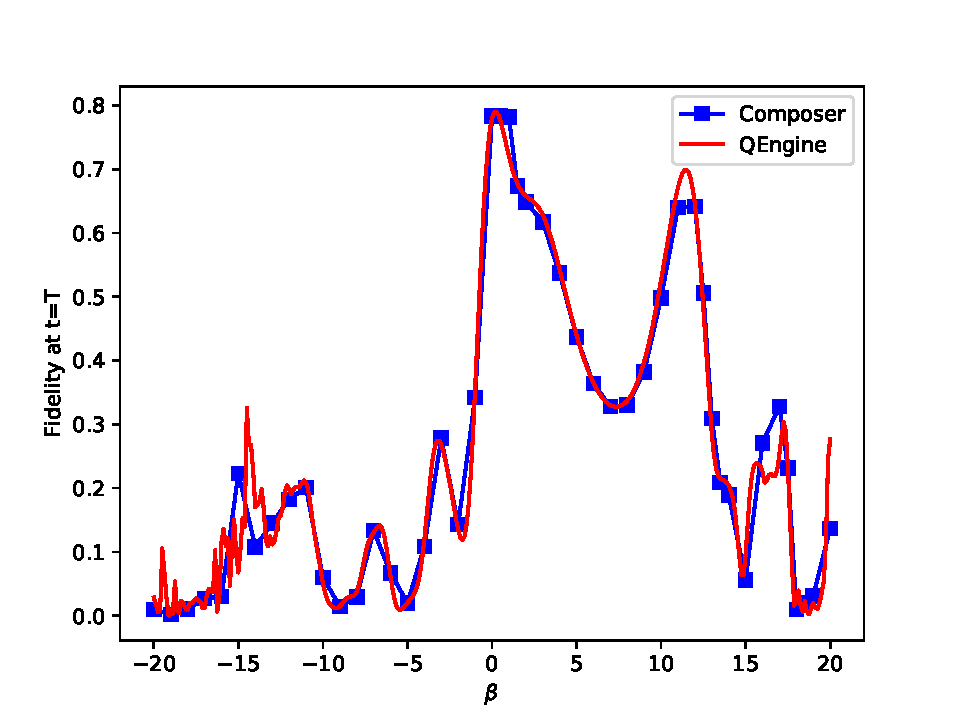
\includegraphics[width=\columnwidth]{graphics/qengine/comparison.pdf}
	\caption{Comparison of the results obtained using Composer and the QEngine to solve the same problem.}
	\label{fig:QEngine_nonOPt}
\end{figure}

In order to explain this difference in behavior, the energies of the first 3 energy eigenstates were calculated in the QEngine and compared with those calculated and plotted in Fig. \ref{fig:energyLevels}. The difference between the Composer energy estimate and the QEngine estimate is plotted in Fig. \ref{fig:QEngine_energydiff}. As can be seen there are small differences between the energies calculated by the 2 tools. This could explain why we observe the difference in fidelity shown in Fig. \ref{fig:QEngine_nonOPt}, since this indicates that the initial and final states are not exactly the same in both programs and thus we would expect them to evolve differently in time.\\

\begin{figure}
	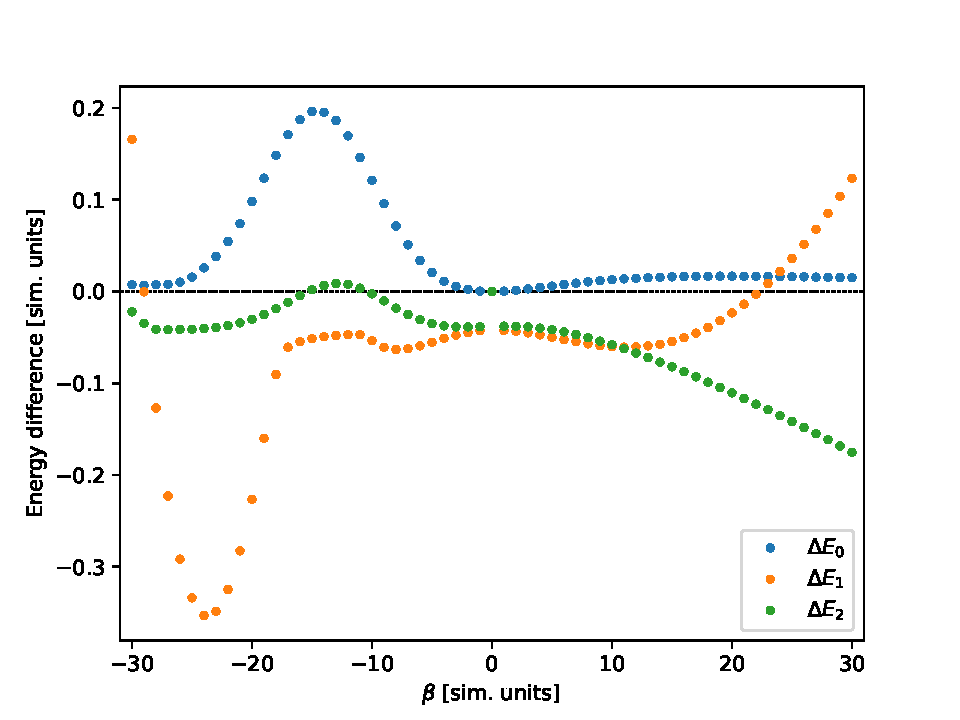
\includegraphics[width=\columnwidth]{graphics/stateAnalysis/energyDiffQEngineComp.pdf}
	\caption{The energy difference between Composer and QEngine for the same system as shown in Fig. \ref{fig:energyLevels} (\textit{A1} in Appendix \ref{App:System-params}). The striped black line marks $\Delta E=0$.}
	\label{fig:QEngine_energydiff}
\end{figure}

Despite this apperent difference in behavior between the 2 tools, the advantages of using QEngine for quantum control optimization and initial seed exploration is demonstrated with the following setup. Firstly, the system is set up using the \textit{exact} same parameters as in the QM2 \textit{Shake Up} (See Appendix \ref{App:System-params}) since it is possible to set the kinetic factor $\kappa$ to any value (Remember that in Composer $\kappa$ is locked to $0.5$) and so no conversion is necessary. Furthermore, the control time was varied between $0.25 ms$ and $1.25 ms$ in steps of $1/32 ms$. With the control durations set, an initial seed 
\begin{equation}
	u_{init}(t) = \sin(2\pi t/T)
\end{equation}
was set. From this seed, 3 new seeds were derived from $u_{init}$ but with added random noise. The noise was set to be a random number in the interval $[-0.7, 0.7]$ and was added to each point of the initial control. Each of these noisy seeds was then optimized using all three optimizers until the step size $\alpha_k$ fell below $10^{-8}$. The resulting infidelity of these optimized solutions are shown in Fig. \ref{fig:QEngine_noise}, where the best results from Composer in Fig. \ref{fig:Clustering} have been included for reference. From this one seed with added noise, it is possible to calculate many more datapoints and optimize seeds to reach better fidelities than what is possible in Composer, even when \proc{Grape} does the optimization. This is most likely a result of having no iteration cap on the optimizer in the QEngine, instead only having a lower bound on the step size taken each iteration. This outperformance of Composer does come at the cost of a considerable computation time, in this case around $10$ hours, to run the code on a laptop with a $1.51$ GHz CPU.

\begin{figure}
	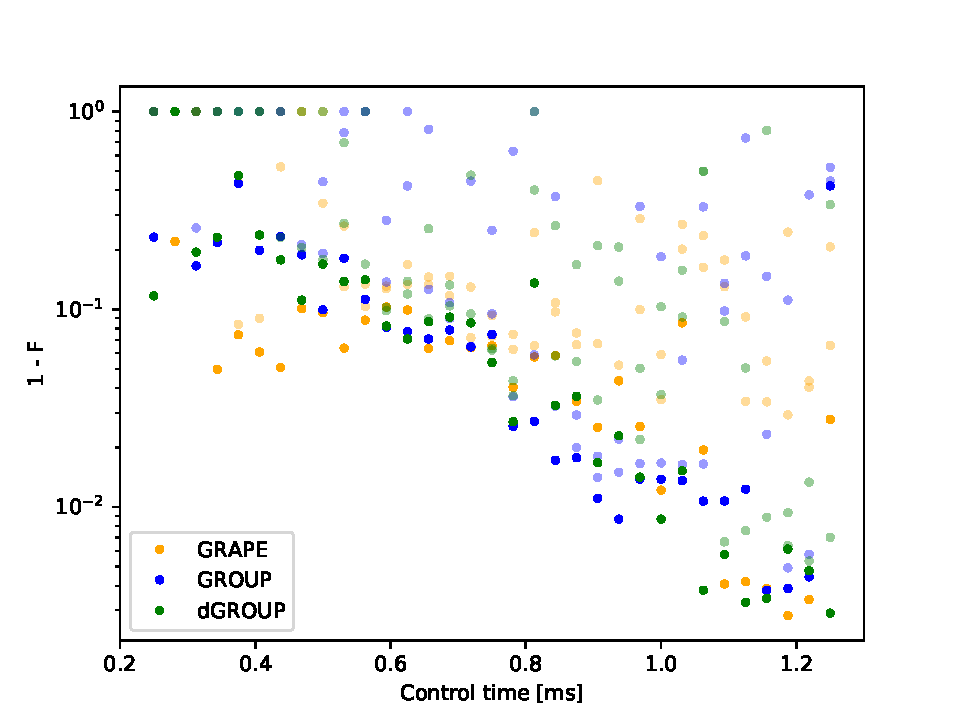
\includegraphics[width=\columnwidth]{graphics/qengine/noiseDemoInf.pdf}
	\caption{Infidelities of solutions optimized using each of the 3 optimizers available in the QEngine. All seeds are generated from the same control function, $u_{init}$, where random noise is then added before optimization. }
	\label{fig:QEngine_noise}
\end{figure}

\section{Comparison}\label{sec:comparison}
As has been demonstrated, QEngine offers several advantages to Quantum Composer with respect to flexibility and computational power. However, this does not mean that the QEngine should be used for every problem. Quantum Composer makes it very easy to set up a desired system, run a simulation on that system and get the system plotted as the system evolves. This makes it preferable to use Composer when one wants to visually and (more or less) playfully explore the behavior of a system as the different parameters are tuned up or down.

Here, I will attempt to list some of the pros and cons of both tools.
\begin{itemize}
	\item[] \textbf{QEngine} 
	\item[\bf+] Flexible and customizable
	\item[\bf+] 3 Optimization algorithms
	\item[\bf+] Superior data gathering capabilities
	\item[\bf{--}] Data must be plotted seperately
	\item[\bf{--}] Data gathering can be \textit{very} time consuming
	\item[\bf{--}] Steep learning curve
	\item[\bf{--}] Difficult installation process
\end{itemize}

\begin{itemize}
	\item[] \textbf{Quantum Composer} 
	\item[\bf+] Many visualization options
	\item[\bf+] Intuitive to explore a given system
	\item[\bf+] Graph node to drag out a control function
	\item[\bf+] Simulating and optimizing is usually fast
	\item[\bf{--}] Limited flexibility and customization
	\item[\bf{--}] Most types of data must be manually gathered
	\item[\bf{--}] Some types of data cannot be exported from the program at all
\end{itemize}
%TODO Cite Composer Cook book somewhere in this paragraph and mention that my conclusions are very similar to those found therein 
Based on the considerations above it is concluded that Quantum Composer is preferable to use as an exploration tool. It is fast to set up, relatively easy to use and most importantly, it is very good at visualizing the simulation through its different kinds of plotting nodes. An example of this exploration could be a physicist trying to simulate an experiment to get a feeling for what kind of settings the experimental apparatus should be capable of. With the current state of Quantum Composer, I find it advantageous to use the QEngine for any kind of simulation where more than around 15 datapoints are desired. While the QEngine has a vastly steeper learning curve, it is designed to easily generate large amounts of data using computationally efficient calculations. It should also be mentioned that, in my personal opinion, having worked or used Composer before working with the QEngine might have smoothed the learning curve of using the QEngine. This is because many of the nodes in Composer correspond to a single class in the QEngine library and so one can use the intuition of how the nodes are connected in Composer to find out how to set up a system in the QEngine. The example files provided with the library are also of great help to get started.\\
%TODO Mention in paragraph above that Composer is build on top of Qengine


It could be advantageous to combine the playful, visual and fast elements that Composer has, with the more systematic, flexible and superior data gathering of the QEngine. One way to possible exploit the best of both these tools could be to use Quantum Composer for globally exploring a given system through the intuitive and playful graph control node. Any promising candidates for good seeds could be exported from Composer in the \texttt{.csv} format to be read by a QEngine script, where noise and other more local optimization approaches could be utilized.

These considerations also give rise to a number of suggestions for desirable features for Quantum Composer in order to make it more attractive to use as an expert tool. Most of these points are a result of a brainstorming/discussion session with Shaeema Ahmed (Aarhus University) and Tiantian Zhang (TU Vienna).

\begin{itemize}
	\item[] \textbf{Desirable features for Quantum Composer} 
	\item Conversion of real world data to dimensionless input scalars
	\item Exportable control functions to potentially be used in experiments
	\item Save data even when for-loops have run
	\item Import control functions from an experiment
	\item Enhance data gathering capabilities all around
	\item Select a time range for control durations
	\item Feed analytical control functions to \proc{Grape} optimizer
	\item Add noise to the control function
	\item A more detailed description of how to use the GPE spectrum node
	\item Undo and redo buttons
	\item An ability to automate data gathering, including exporting data
\end{itemize}

\section{Discussion}\label{sec:discussion}
%As explained in section \ref{sec:strats}, the Quantum Composer software in this workshop allows for 2 different ways to construct control functions. While both methods have been used to explore the behavior of BECs subject to a controlled potential, the files only allow optimization of control functions made using the graph method.

%While the graph method has its advantages as discussed above, the analytical function approach likewise has advantages that could be combined with $\proc{Grape}$. Having multiple approaches to the optimization problem would most likely be beneficial both from a perspective of understanding and from the perspective of being able to fine tune parameters for generating good seeds.\\

The energy spectrum is generated in Quantum Composer to create wave functions, find energy levels and calculate variances wrt. $\hat{H}_{GPE}$. This generation is subject to some initial guesses that can be tweaked to minimize the variance of any relevant states, thus ensuring that the simulation will be as accurate as possible. However, it seems to be the case that while one can tweak these guesses to reach low variances (on the order $10^{-8}$ or better) for one set of system parameters (e.g. $x_{max}$, $x_{min}$, $\beta$), it has not been possible to find a set of initial parameters that keep the variance low as the system is altered. This is a relevant source of error as a substantial part of the results in this report describe how $\beta$ changes the system behavior. 

Thus the accuracy of the results could be improved further, in some cases even greatly, by instead of keeping the initial guesses the same as the system was altered, to instead have the guesses re-tweaked to fit the new system. By recalculating the spectrum for each system, it is suspected that different results could be obtained for some figures, most notably Fig. \ref{fig:beta}, \ref{fig:QSL} and \ref{fig:reachable_neg_betas}. This is due to the control function $u_{\mathrm{non-opt}}(t)$ depending on the energy spacing between the first 2 states, $\omega_{01}$, and because the 2 other figures are presumed to be particularly sensitive to sources of error in the calculation of initial and target state.   \\

In addition to the source of error regarding the estimate of the QSL shown in Fig. \ref{fig:QSL}, it is believed that these estimates are higher than what is actually the speed limit for this problem. This is mainly based on the number of \proc{Grape} iterations being set to the relatively low value of $100$ iterations, where it would be beneficial to instead have it several times higher, e.g. $750$ or $1000$ iterations. The number of iterations was set this low due to the lack of automated data gathering in Composer. This is particularly problematic when optimizing systems with a duration around the QSL of the problem, since the optimization landscape is relatively flat and so the step size $\alpha_k$ has to be lower in order for \proc{Grape} to properly traverse it. This means that while it will take a large number of iterations to reach a height of $0.99$, it will most likely be possible for values lower than those currently found. 

Likewise it should also be kept in mind that only a very limited part of the ``control space'' has been explored so far, and so it would most likely be a matter of doing a more persistant search to find a lower QSL for one or more of the $\beta$s examined. This is one of the places where it would be very interesting to be able to add random noise to a control seed as one can do in the QEngine, as this would most likely increase the exploration of the local optimization landscape that the initial seed has ``globally'' pointed out. This could hopefully lead to a similar situation as the one seen in Fig. \ref{fig:QEngine_noise}, where the optimized ``noisy'' seeds were able to outperform the controls optimized in Composer.\\

%TODO Notice that the control limitations from QM2 system were not implemented in my runs with the QEngine

Throughout both the exploration and data collection parts of this challenge, the control functions that have been used have for the most part been simple harmonic functions like $A\sin(\pi t/T)$ or other simple approaches such as the function seen in Fig. \ref{fig:Controls} (b).


As described in section \ref{subsec:numericalLimitations}, some of the ways to explore this problem are blocked by numerical instabilities. This could possibly be fixed by increasing the number of timesteps, which is currently $501$, since the smaller the timestep used, the better an approximation each step forwards in time becomes. This might mean that the GPE spectrum would have to be recalculated to minimize the variance of important states, but also mean an increased computational cost of each simulation.


\section{Conclusion}\label{sec:conclusion}
%TODO Update me 
%Composer
The backbone of the results in this report have been generated in Quantum Composer. The workflow of using this amateur tool for data gathering and visualization has been described and visualized. %Numerical stuff
The numerical boundaries of Composer have been demonstrated and their implications for exploring the challenge have been discussed. Likewise the performance and numerical accuracy of different grid sizes have been estimated their results on the performance/accuracy trade-off discussed.

% Results
It has been demonstrated that the behavior of BECs are sensitive to the parameters $\beta$ and $T$. As it has been shown in Fig. \ref{fig:HO}, this changed behavior compared to a single particle can be beneficial and capable of reaching higher fidelity than is otherwise possible. On the other hand it is also apparent that $\beta$ introduces an unpredictability into the system as well as numerical inaccuracy of the Hamiltonian eigenstates. It has also been shown that the $\beta$ term in \eqref{eq:Hbec} increases the QSL up to a estimated value of 2 times that of a single particle for the case $\beta=25$. It was also attempted to cluster the performance of $\cos(k\pi t/T)$ control seeds to the frequency $k$, although the data shown in Fig. \ref{fig:Clustering} shown that the seed frequency and optimized performance are not connected in a straightforward manner. What seems more promising is analyzing the number shakes in the optimized solutions and clustering these. The robustness of some optimized solutions have been explored both regarding a scaled potential and a scaled atomic interaction, as is shown in Fig. \ref{fig:robustness}.

%Strats
Some strategies involving choosing a control function have also been explored. The differences, advantages and disadvantages of using either an analytical function node or a graph node to determine the control function have been discussed. This includes how varying $T$ affects the control function, as has been illustrated on figures \ref{fig:funcAppr} and \ref{fig:graphAppr}. Finally, 2 concrete strategies for determining the QSL in this problem have been explained, both using the graph node to create a control function.

%QEngine
The QEngine has been used to generate data that illustrate how it differs from using Quantum Composer. The results indicate that without some more tweaking and a better understanding of to replicate a system even more accurately, the results generated by the QEngine and in Composer will differ slightly as was seen in Fig. \ref{fig:QEngine_energydiff}. It was also shown that one can use the QEngine to further improve on Composer results, where seeds with random noise were optimized using all 3 optimizers available in the QEngine. While the state evolution in Composer and QEngine seems to differ slightly, it should be noted that the QEngine is able to match or outperform the best results from the different seeds used in Composer, by using a single seed with added random noise and optimization by different algorithms and no iteration cap.

%Comparison
Based on the work done using both tools, their pros and cons have been discussed and suggestions for where it is advantageous to use one tool over the other have been provided, as well as when it might be useful to use both tools for the same problem.

Furthermore, a list of desirable additions to Quantum Composer has been added. The implementation of these features would hopefully make the tool a more effective tool for expert-use, where customization, flexibility and automated data gathering features are highly valued.

%Perspectives
Future aspects of this problem that could be interesting to research include:
\begin{itemize}
	\item Further explorations of the possible seeding strategies in the QEngine
	\item A more in-depth explanation of the 3 optimization algorithms \proc{Grape}, \proc{Group} \& d\proc{Group}.
\end{itemize}

\bibliography{thebibliography}

\appendix
\section{System parameters}\label{App:System-params}
%Generally
Generally when doing numerical calculations it can be useful to rescale small or large quantities like $\hbar$ or $M_{Sun}$ to a new size in order to avoid problems caused by finite precision memory and rounding errors. In this report the relevant quanteties for rescaling are
\begin{align}
	x_{SI} = \mu_{length} x, \quad t_{SI} = \mu_{time} t, \quad V_{SI} &= \mu_{energy} V
\end{align}
Here $\mu_{energy}$ is chosen as 
\begin{equation}
	\mu_{energy} = \frac{\hbar^2}{2\kappa m \chi^2}
\end{equation}
where $\kappa$ is the \textit{kinetic factor}. 

One can freely define 2 of the 3 quantities $\{ \mu_{length},\mu_{time},\kappa \}$ and the remaining quantity will follow. Throughout the report the mass is taken as $\mu_{mass}=m_{Rb87}$ and we require $\mu_{energy} = \hbar / \tau$ in order to get dimensionless equations of motion, where $\hbar = m = 1$. Unless otherwise stated, the grid size used was $n_x = 256$. \\
%TODO Find out what the x bounderies were at different levels, some pm 6, while other pm 2

%Quadratic
\textit{System A1}: Units are chosen as
\begin{subequations}
	\begin{gather}
		\mu_{length} = 1 \mu\text{m}, \quad \kappa = 0.5 \label{eq:sys_a1_units_choice}\\
		\Rightarrow \mu_{time} = 2\kappa \mu_{mass}\mu^2_{length} / \hbar = 1.3699\text{ ms} \label{eq:sys_a1_units_notChoice}
	\end{gather}
\end{subequations}
with potential 
\begin{equation}
	V(u) = a(x-u)^2
	\label{eq:sys_a1_potential}
\end{equation}
where $a = 50$. The value of $\beta$ was varied in this system. \\

%Quartic
\textit{System B1}: Units are chosen in the same way as in Eqs. \eqref{eq:sys_a1_units_choice}-\eqref{eq:sys_a1_units_notChoice}. The potential from Eq. \eqref{eq:sys_a1_potential} is modified with a quartic term
\begin{equation}
	V(u) = a(x-u)^2 + b(x-u)^4
	\label{eq:sys_b1_potential}
\end{equation} 
with $b = 128$. $\beta$ was also varied in this system. \\
%QM2 Shake Up
\textit{Shake up} level in Ref. \cite{QM2Paper}:
\begin{subequations}\label{eq:sys_QM2_units}
	\begin{gather}
		\mu_{length} = 1 \mu\text{m}, \quad \mu_{time} = 1\text{ ms} \label{eq:sys_QM2_units_choice}\\
		\Rightarrow \kappa = \hbar \mu_{time} / (2 \mu_{mass} \mu^2_{length}) = 0.36537 \label{eq:sys_QM2_units_notChoice}
	\end{gather}
\end{subequations}
The potential used was
\begin{equation}
	V(u) = \sum\limits_{r = 2,4,6} = p_r (x - u)^r
	\label{eq:sys_QM2_potential}
\end{equation} 
with coefficients and interaction strength
\begin{subequations}\label{eq:sys_QM2_params}
	\begin{align}
		p_2& = 65.8392,& p_4& = 97.6349, \\
		p_6& = -15.3850,& \beta& = 1.8299
	\end{align}
\end{subequations}

%From QM2 -> Composer
\textit{Composer implementation of QM2 Shake up}:
Since Quantum Composer has a locked choice of $\kappa = 0.5$, it is necessary to rescale the units from the Quantum Moves 2 level \textit{Shake Up} in order to simulate the same system in Composer. The scaling factor is $0.5/0.36537 \approx 1.368$ and yields the following transformation of Eqs. \eqref{eq:sys_QM2_units}-\eqref{eq:sys_QM2_params}

\begin{subequations} \label{eq:sys_compQM2_params}
	\begin{align}
		\kappa& = 0.5,& \mu_{time}& =1.368\text{ ms}, \\
		\beta& = 2.5042,& p_2& = 90.0994, \\
		p_4& = 133.611,& p_6 &= -38.5267
	\end{align}
\end{subequations}

\end{document}
